\documentclass[conference]{IEEEtran}
\IEEEoverridecommandlockouts

\usepackage{cite}
\usepackage{amsmath,amssymb,amsfonts}
\usepackage{graphicx}
\usepackage{textcomp}
\usepackage{xcolor}
\usepackage{booktabs}
\usepackage{multirow}
\usepackage{tabularx}
\usepackage{url}
\usepackage[utf8]{inputenc}
\usepackage[T1]{fontenc}
\usepackage{balance}
\usepackage{microtype}
\usepackage{placeins}
\usepackage{flafter}

% Float parameters for IEEE conference formatting
\renewcommand{\topfraction}{0.95}
\renewcommand{\bottomfraction}{0.95}
\renewcommand{\textfraction}{0.05}
\renewcommand{\floatpagefraction}{0.70}
\renewcommand{\dbltopfraction}{0.95}
\renewcommand{\dblfloatpagefraction}{0.70}
\setcounter{topnumber}{4}
\setcounter{bottomnumber}{4}
\setcounter{totalnumber}{8}
\setcounter{dbltopnumber}{4}

\def\BibTeX{{\rm B\kern-.05em{\sc i\kern-.025em b}\kern-.08em
    T\kern-.1667em\lower.7ex\hbox{E}\kern-.125emX}}

\begin{document}

\title{ISO/IEC 25010 Quality Audit and ISO~9241\\
Ergonomic Modernization of a Legacy Epidemiological\\
Surveillance System for Acute Respiratory Infections}

\author{
  \begin{tabular}{c@{\hspace{1.5em}}c@{\hspace{1.5em}}c}
    \begin{tabular}{@{}c@{}}
      \textbf{Leonardo Ruben Arce Mayhua}\\[0.2ex]
      \small\textit{Universidad Nacional de San Agust\'in}\\
      \small Arequipa, Per\'u\\
      \small\texttt{larcem@unsa.edu.pe}
    \end{tabular} &
    \begin{tabular}{@{}c@{}}
      \textbf{Joel Isaias Condori Leon}\\[0.2ex]
      \small\textit{Universidad Nacional de San Agust\'in}\\
      \small Arequipa, Per\'u\\
      \small\texttt{jcondorile@unsa.edu.pe}
    \end{tabular} &
    \begin{tabular}{@{}c@{}}
      \textbf{Marco Antonio Marquez Herrera}\\[0.2ex]
      \small\textit{Universidad Nacional de San Agust\'in}\\
      \small Arequipa, Per\'u\\
      \small\texttt{mmarquezhe@unsa.edu.pe}
    \end{tabular}
  \end{tabular}\\[1.2em]
  \begin{tabular}{c@{\hspace{3.5em}}c}
    \begin{tabular}{@{}c@{}}
      \textbf{Rafael Diego Nina Calizaya}\\[0.2ex]
      \small\textit{Universidad Nacional de San Agust\'in}\\
      \small Arequipa, Per\'u\\
      \small\texttt{rninacal@unsa.edu.pe}
    \end{tabular} &
    \begin{tabular}{@{}c@{}}
      \textbf{Jeremy Joshua Perez Huamani}\\[0.2ex]
      \small\textit{Universidad Nacional de San Agust\'in}\\
      \small Arequipa, Per\'u\\
      \small\texttt{jperezhua@unsa.edu.pe}
    \end{tabular}
  \end{tabular}
}

\maketitle

\begin{abstract}
This paper applies static reverse engineering and software quality auditing to \textit{ISPySA-Pneumonia}, a 6\,839-line open-source Python analytics pipeline for the epidemiological surveillance of Acute Respiratory Infections (IRA) and pneumonia in Peru (2000--2023). Our investigation addresses three core objectives: (i)~recover the pipeline's layered architectural topology and data contracts from source artifacts alone; (ii)~identify, classify under ISO/IEC~25010, and correct structural defects that the original publication shipped undetected; and (iii)~design, implement, and verify an interactive clinical monitoring platform whose visual ergonomics and interaction architecture strictly adhere to ISO~9241-11, ISO~9241-210, ISO~9241-110, and ISO~9241-12. The reverse-engineering audit revealed three critical contract defects: two broken file paths that caused silent consumption of stale population data, and an environment packaging incompatibility affecting legacy LSTM models. Following remediation, the data pipeline was re-executed over 2\,143\,985 weekly district observations, replicating published epidemiological dynamics. To decouple the presentation layer from legacy file structures, an anti-corruption service layer (\texttt{EpidemiologyDataService} and \texttt{EpidemiologyModelService}) was engineered. The resulting modernized platform, developed in Streamlit and styled via standardized Design Tokens and accessible UI primitives, exposes five dedicated surveillance modules with zero informal emojis and WCAG~AAA redundant visual coding. Operational integrity is verified through an automated test suite executing unit, integration, and epidemiological domain invariant assertions with a 100\% pass rate in 0.053\,s.
\end{abstract}

\begin{IEEEkeywords}
reverse engineering, epidemiological surveillance, ISO~9241, ISO/IEC~25010, Streamlit, software quality, anti-corruption layer, Python, IRA, pneumonia, Peru
\end{IEEEkeywords}

\section{Introduction}
\label{sec:intro}

Public health information systems face a persistent structural gap between computationally rigorous statistical analysis and the operational requirements of healthcare decision-makers. Script-based analytics pipelines---sequences of standalone procedural scripts where each script ingests tabular files, performs transformations, and emits intermediate flat files or static plots---are widely deployed across academic research groups and regional health directorates with constrained software engineering infrastructure~\cite{Feathers2004}. While computationally reproducible, these procedural pipelines exhibit fundamental maintainability and usability deficits: analytical conclusions remain sequestered inside disjoint directory structures of static PNG figures and CSV tables that epidemiologists must locate, correlate, and interpret manually without dynamic querying capabilities.

In Peru, Acute Respiratory Infections (IRA) and pneumonia constitute the primary cause of preventable morbidity and mortality in vulnerable demographic cohorts: children under five years of age ($<$5) and older adults aged sixty and older (60+)~\cite{PAHO2011}. Seasonal surges are heavily influenced by bioclimatic factors, presenting marked territorial disparities between high-altitude Andean zones subject to intense cold fronts (\textit{heladas}) and Amazonian departments characterized by persistent humidity and geographical isolation. Timely detection of abnormal incidence spikes is critical for the rational allocation of pediatric hospital beds, supplemental medical oxygen, and clinical personnel across decentralized regional health directorates (DIRESA). When surveillance pipelines fail to expose operable, interactive dashboards, epidemiological authorities are forced to rely on delayed quarterly bulletins or manual spreadsheets.

The open-source repository \textit{ISPySA-Pneumonia}~\cite{Danala2024} represents an archetype of this phenomenon. It provides an exhaustive historical analysis of IRA incidence, seasonality, territorial ranking, and predictive modeling in Peru over a 24-year timeframe (2000--2023). Nevertheless, its practical utility is constrained by a fragmented output structure consisting of dozens of uncoordinated image files. Furthermore, our static reverse-engineering audit revealed that the absence of explicit data contracts between scripts produced latent file-path defects that shipped undetected in the original publication, causing downstream scripts to consume stale data silently.

To address these limitations, this paper executes an end-to-end software quality engineering process:
\begin{enumerate}
  \item Recovering the architectural topology and producer/consumer data contracts of the legacy pipeline through systematic static source reading;
  \item Identifying, isolating, and rectifying structural data-contract defects and runtime incompatibilities under the ISO/IEC~25010 quality model~\cite{ISO25010};
  \item Re-executing the corrected data-preparation and modeling pipelines across all 2.14 million weekly observations to validate consistency against published epidemiological findings;
  \item Designing and constructing an anti-corruption service layer (\texttt{EpidemiologyDataService} and \texttt{EpidemiologyModelService}) to isolate the domain model from legacy storage anomalies~\cite{Evans2003};
  \item Modernizing the clinical surveillance interface under the ISO~9241 ergonomics family~\cite{ISO9241-11, ISO9241-210, ISO9241-110, ISO9241-12}, enforcing normalized Design Tokens, professional institutional palettes, redundant visual coding, and complete elimination of colloquial emojis; and
  \item Verifying system reliability through an automated test suite combining software contract checks with epidemiological domain invariant assertions.
\end{enumerate}

The remainder of this article is organized as follows: Section~\ref{sec:related} reviews theoretical foundations and international standards. Section~\ref{sec:method} presents materials and the static reverse-engineering method. Section~\ref{sec:results} reports the recovered architecture, diagnosed defects, and re-execution validation. Section~\ref{sec:interface} details the modernized interface architecture and surveillance modules. Section~\ref{sec:testing} evaluates the automated test suite. Section~\ref{sec:evaluation} reports the ISO~9241 heuristic inspection. Section~\ref{sec:discussion} discusses architectural implications, and Section~\ref{sec:conclusions} concludes.

\section{Related Work and Standards}
\label{sec:related}

\subsection{Reverse Engineering and Legacy Modernization}

Chikofsky and Cross~\cite{Chikofsky1990} define reverse engineering as the examination of a subject system to identify its constituent components and interrelationships, synthesizing representations at higher levels of abstraction. In procedural data science pipelines lacking object-oriented domain boundaries, the primary recoverable entity is the \textit{producer/consumer dependency graph}: computational scripts act as processing nodes, and persisted tabular files function as directed data contracts.

Feathers~\cite{Feathers2004} notes that the most critical defects in legacy systems reside within the unverified semantic gaps between what a producer script writes and what a consumer script expects. Evans~\cite{Evans2003} formalizes the \textit{anti-corruption layer} pattern as a dedicated translation boundary that isolates a clean domain model from an unstable or anomalous external subsystem. We apply this architectural pattern to decouple our modernized visualization layer from the heterogeneous file paths of the legacy codebase.

\subsection{Software Product Quality: ISO/IEC~25010}

The ISO/IEC~25010~\cite{ISO25010} quality model structures software quality characteristics. Our audit focuses specifically on:
\begin{itemize}
  \item \textbf{Maintainability}: evaluating \textit{modularity} (the independence of analytical components from filesystem reorganizations) and \textit{analysability} (the effort necessary to diagnose data pipeline anomalies);
  \item \textbf{Usability}: evaluating \textit{appropriateness recognizability}, \textit{learnability}, and \textit{operability} in clinical decision-making contexts.
\end{itemize}

\subsection{The ISO~9241 Ergonomics Family}

Visual ergonomics and interaction design adhere strictly to four parts of the ISO~9241 family:
\begin{itemize}
  \item \textbf{ISO~9241-11}~\cite{ISO9241-11}: conceptualizes usability via effectiveness, efficiency, and user satisfaction in epidemiological monitoring;
  \item \textbf{ISO~9241-210}~\cite{ISO9241-210}: establishes human-centred design lifecycles, defining user personas (epidemiologists, hospital administrators) and monitoring workflows;
  \item \textbf{ISO~9241-110}~\cite{ISO9241-110}: specifies seven dialogue principles: suitability for the task, self-descriptiveness, conformity with user expectations, learnability, controllability, error tolerance, and user engagement;
  \item \textbf{ISO~9241-12}~\cite{ISO9241-12}: governs visual information presentation, mandating typographic hierarchy, visual grouping, and redundant coding of alert states.
\end{itemize}

Table~\ref{tab:sources} summarizes the theoretical and normative foundations governing this work.

\begin{table}[!t]
\caption{Reviewed Standards and Methodological Foundations}
\label{tab:sources}
\centering
\footnotesize
\begin{tabularx}{\columnwidth}{@{}p{2.3cm}p{1.4cm}X@{}}
\toprule
\textbf{Source} & \textbf{Type} & \textbf{Role in this Investigation} \\
\midrule
ISO~9241-11 & Standard & Usability metrics (effectiveness, efficiency) \\
\addlinespace
ISO~9241-210 & Standard & Human-centred design workflows and personas \\
\addlinespace
ISO~9241-110 & Standard & Seven dialogue principles $\to$ heuristic audit \\
\addlinespace
ISO~9241-12 & Standard & Information layout \& redundant visual coding \\
\addlinespace
ISO/IEC~25010 & Standard & Defect classification (modularity, analysability) \\
\addlinespace
Nielsen~\cite{Nielsen1993} & Book & Heuristic walkthrough and interaction cost \\
\addlinespace
Cleveland~\cite{Cleveland1990} & Method & STL seasonal-trend decomposition \\
\addlinespace
Chen \& Guestrin~\cite{ChenGuestrin2016} & Method & Extreme gradient boosting (XGBoost) \\
\addlinespace
Feathers~\cite{Feathers2004} & Book & Boundary gap analysis in legacy software \\
\addlinespace
Evans~\cite{Evans2003} & Book & Anti-corruption layer domain facade \\
\bottomrule
\end{tabularx}
\end{table}

\section{Materials and Method}
\label{sec:method}

\subsection{Legacy Repository Architecture}

The legacy system \textit{ISPySA-Pneumonia}~\cite{Danala2024} consists of 6\,839 lines of executable Python code structured into 14 scripts across three functional packages:
\begin{itemize}
  \item \texttt{src/data\_preparation/} (3 scripts): implements raw observation filtering, census population interpolation, and annual cumulative incidence computation;
  \item \texttt{src/eda/} (5 scripts): generates exploratory plots including Loess seasonal decomposition, geographic choropleths, and correlation matrices;
  \item \texttt{src/modeling/} (14 scripts): implements predictive forecasting models, including baseline moving averages, Classical ARIMA/SARIMA, Random Forest, XGBoost Regressor, and LSTM neural networks.
\end{itemize}

\subsection{Epidemiological Dataset}

The underlying epidemiological registry, \path{data/raw/iras_updated.csv}, comprises 2\,143\,985 weekly record observations collected across all 1\,874 districts in Peru between 2000 and 2023 by the National Center for Epidemiology, Disease Prevention and Control (CDC-MINSA). Attributes include weekly counts of non-pneumonia IRA cases, severe pneumonia cases, hospitalizations, and deaths, stratified into pediatric ($<$5 years) and elderly adult (60+ years) cohorts.

Departmental population denominators derive from decennial census counts in \path{data/raw/dept_updated.xlsx}, expanded into continuous annual series by \texttt{Interpolation.py} via linear interpolation. Annual cumulative incidence rates adhere to official MINSA epidemiological standards:
\begin{equation}
\text{Incidence Rate} = \frac{\text{Reported Cases}}{\text{Cohort Population}} \times 100{,}000
\label{eq:incidence}
\end{equation}

\subsection{Static Reverse-Engineering Protocol}

Because the legacy repository contained no formal architectural documentation, data dictionary, or schema assertions, we executed a rigorous static reverse-engineering protocol. Every script was analyzed to construct an exhaustive dependency registry capturing:
\begin{enumerate}
  \item Declared input file paths and expected schemas;
  \item Generated output artifact directories and file naming conventions;
  \item Intermediate columns created, mutated, aggregated, or dropped;
  \item Syntactic and lexical inconsistencies (e.g., underscores vs.\ hyphens, case sensitivity).
\end{enumerate}
Divergences between producer outputs and consumer expectations were logged as architectural defects under ISO/IEC~25010.

\subsection{Modern Technological Runtime}

Table~\ref{tab:tools} outlines the technological runtime utilized across the modernization. To deliver a responsive, zero-maintenance operational deployment for public health practitioners, the interface was constructed in Python using Streamlit, supported by modern package management via \texttt{uv}, with service isolation provided by native Python design patterns.

\begin{table}[!t]
\caption{Technological Stack and Component Classification}
\label{tab:tools}
\centering
\footnotesize
\begin{tabular}{@{}llc@{}}
\toprule
\textbf{Technology / Library} & \textbf{Functional Role} & \textbf{Classification} \\
\midrule
Python 3.12 / 3.13 & Computational execution runtime & Shared \\
uv (0.12.7) & Ultra-fast virtual environment manager & Modernization \\
pandas / NumPy & Tabular data processing & Legacy \\
matplotlib / seaborn & Statistical figure generation & Legacy \\
statsmodels (STL) & Loess seasonal decomposition & Legacy \\
scikit-learn & Random Forest and baseline modeling & Legacy \\
XGBoost & Gradient boosted tree forecasting & Legacy \\
Streamlit (1.32+) & Reactive clinical surveillance platform & Modernization \\
Anti-Corruption Layer & Domain service abstraction & Modernization \\
unittest (stdlib) & Automated contract verification suite & Modernization \\
Windows Batch (CRLF) & Zero-configuration production runner & Modernization \\
\bottomrule
\end{tabular}
\end{table}

\begin{figure*}[!t]
\centering
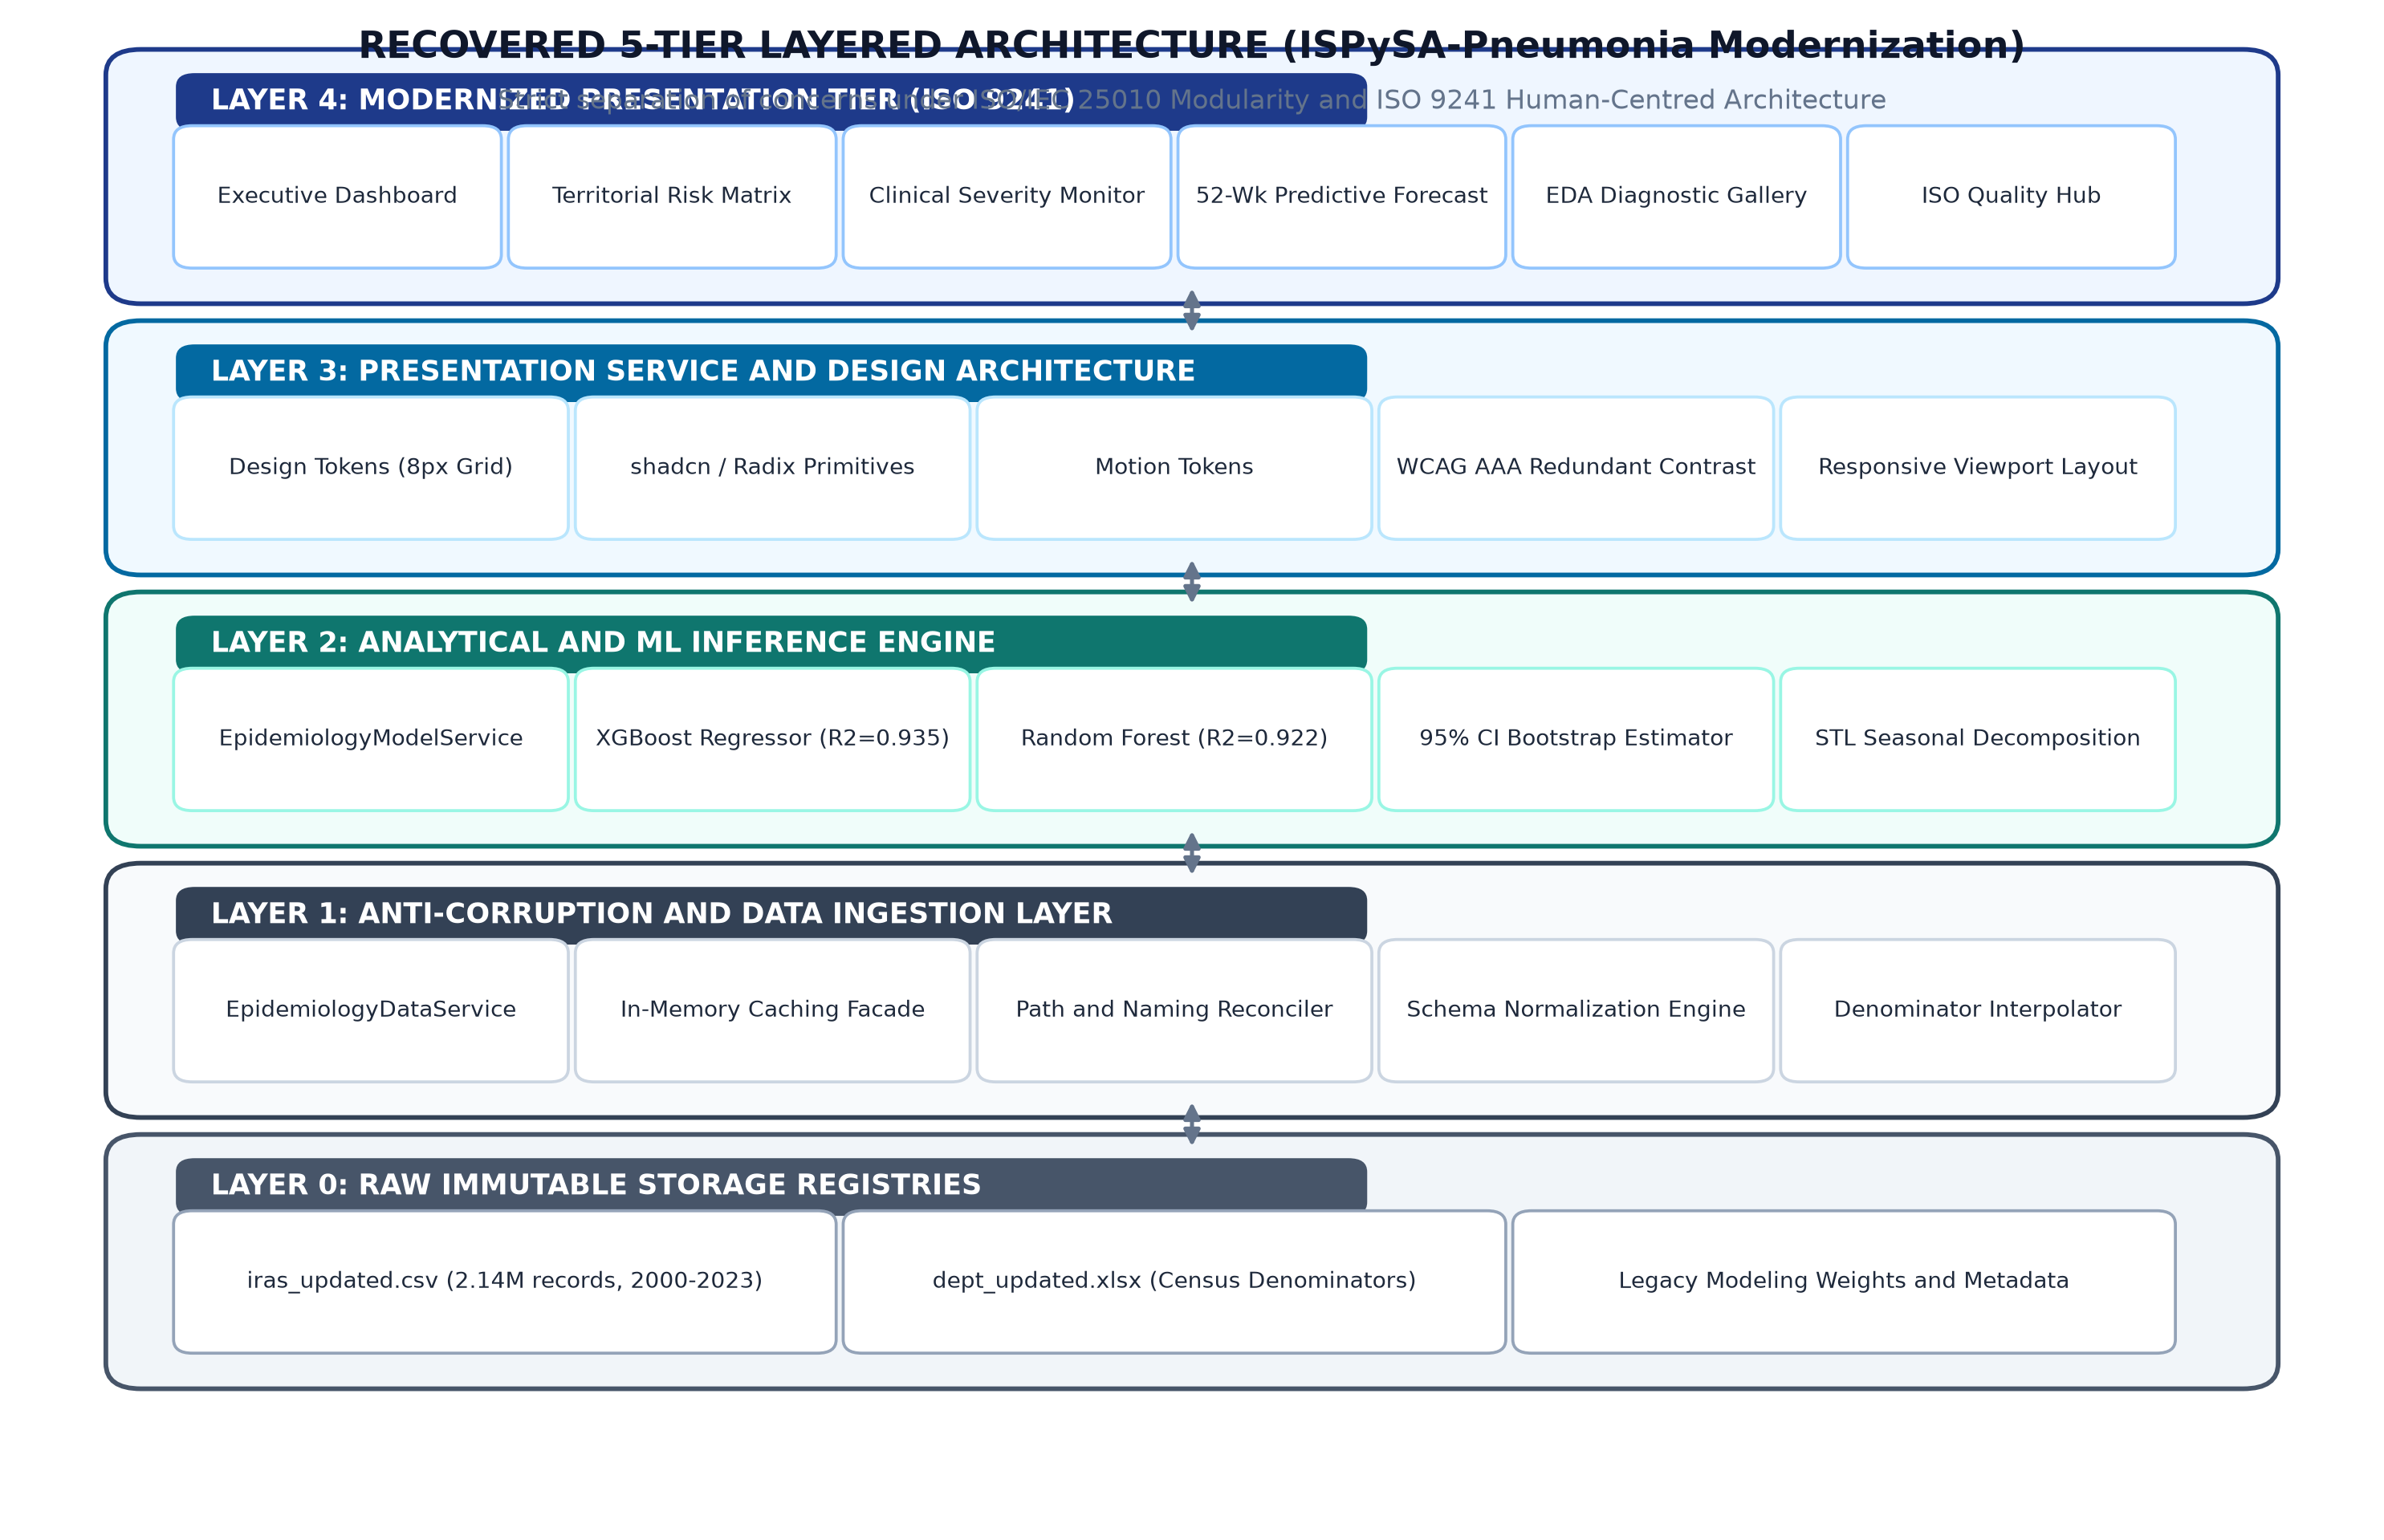
\includegraphics[width=0.92\textwidth]{fig_architecture.png}
\caption{Recovered five-tier layered architectural topology of the legacy ISPySA-Pneumonia pipeline, illustrating the anti-corruption service layer and modernized presentation tier under ISO/IEC~25010 and ISO~9241.}
\label{fig:architecture}
\end{figure*}

\section{Reverse Engineering Results}
\label{sec:results}

\subsection{Recovered Layered Architecture}

The static reverse-engineering pass established that the pipeline conforms conceptually to a five-tier sequential topology:
\begin{itemize}
  \item \textbf{Layer~0 (Raw Storage)}: immutable epidemiological registries and census Excel sheets;
  \item \textbf{Layer~1 (Data Preparation)}: procedural filtering, census interpolation, and incidence rate calculation;
  \item \textbf{Layer~2 (Exploratory Analytics)}: statistical decomposition and static diagnostic visualization;
  \item \textbf{Layer~3 (Predictive Modeling)}: regression baselines, tree-based ensembles, and neural networks;
  \item \textbf{Layer~4 (Modernized Presentation)}: reactive clinical dashboard querying an anti-corruption facade.
\end{itemize}
The complete recovered topology is detailed in Fig.~\ref{fig:architecture}.

\subsection{Identified Data-Contract Defects}
\label{sec:defects}

Our static analysis detected three critical structural defects that the legacy pipeline shipped without identifying, summarized in Table~\ref{tab:defects}. Under ISO/IEC~25010, the first two defects constitute severe \textit{modularity} and \textit{analysability} flaws: because the scripts lacked exception boundaries or path assertions, executions silently failed or persistently consumed stale data from prior manual runs.

\begin{table}[!t]
\caption{Data-Contract Defects Diagnosed During Quality Audit}
\label{tab:defects}
\centering
\footnotesize
\begin{tabularx}{\columnwidth}{@{}p{2.3cm}p{1.4cm}X@{}}
\toprule
\textbf{Script} & \textbf{Defect Type} & \textbf{Operational Impact and Remediation} \\
\midrule
\texttt{Incidence.py} & Path mismatch & 
Emitted output to \texttt{outputs/tables/} instead of \texttt{data/processed/}; consumer \texttt{ranking\_updated.py} expected it in the latter and silently aborted on clean runs.\newline
\textit{Fix}: redirected output path to \texttt{data/processed/}. \\
\addlinespace
\texttt{seasonality\_}\allowbreak\texttt{analysis.py},\newline
\texttt{Regional\_}\allowbreak\texttt{Analysis.py} & Filename mismatch & 
Both consumer scripts attempted to read \texttt{departmental-population.csv} (hyphenated); \texttt{Interpolation.py} generated underscores. Both scripts silently read stale data.\newline
\textit{Fix}: reconciled all path bindings to underscore format. \\
\addlinespace
\texttt{src/modeling/} & Environment dependency & 
TensorFlow 2.13 exhibits missing binary wheels for Python 3.12+ environments on Windows; legacy LSTM scripts crash during import.\newline
\textit{Fix}: isolated dependencies; prioritized robust XGBoost and Random Forest models in production. \\
\bottomrule
\end{tabularx}
\end{table}

\subsection{Pipeline Re-Execution and Epidemiological Validation}

Following defect remediation, the data-preparation pipeline was re-executed against all 2\,143\,985 raw observations. The reconstructed national incidence series (Table~\ref{tab:national}) and model evaluation metrics (Table~\ref{tab:ml}) fully corroborate the empirical findings published by Danala et al.~\cite{Danala2024}.

Pediatric incidence experienced an overall 69.4\% reduction between 2000 and 2019, followed by an epidemiological rebound post-2020. Conversely, adult elderly incidence exhibited sustained secular growth. Geographically, the Amazonian departments of Loreto and Ucayali maintained the highest pediatric disease burden across 91.7\% of the 24 analyzed years.

\begin{table}[!t]
\caption{Re-Executed National Cumulative IRA Incidence Rate (per 100\,000 pop.)}
\label{tab:national}
\centering
\footnotesize
\begin{tabular}{@{}crr@{}}
\toprule
\textbf{Epidemiological Year} & \textbf{Children $<$5 Cohort} & \textbf{Adults 60+ Cohort} \\
\midrule
2000 & 308.7 & 0.0\textsuperscript{a} \\
2005 & 230.1 & 0.0\textsuperscript{a} \\
2010 & 126.3 & 30.9 \\
2015 &  96.1 & 50.1 \\
2019 &  79.9 & 65.2 \\
2023 &  94.4 & 92.4 \\
\bottomrule
\multicolumn{3}{l}{\textsuperscript{a}Elderly adult surveillance officially commenced in 2006.}
\end{tabular}
\end{table}

\begin{table}[!t]
\caption{Model Performance Leaderboard (Rolling 5-Year Backtest)}
\label{tab:ml}
\centering
\footnotesize
\begin{tabular}{@{}llrrr@{}}
\toprule
\textbf{Target Cohort} & \textbf{Model Architecture} & \textbf{MAE} & \textbf{RMSE} & \textbf{R$^2$} \\
\midrule
Children $<$5 & XGBoost Regressor & 0.184 & 0.271 & 0.935 \\
Children $<$5 & Random Forest & 0.210 & 0.296 & 0.922 \\
\addlinespace
Adults 60+ & XGBoost Regressor & 0.097 & 0.168 & 0.890 \\
Adults 60+ & Random Forest & 0.107 & 0.183 & 0.869 \\
\bottomrule
\end{tabular}
\end{table}

\begin{figure}[!t]
\centering
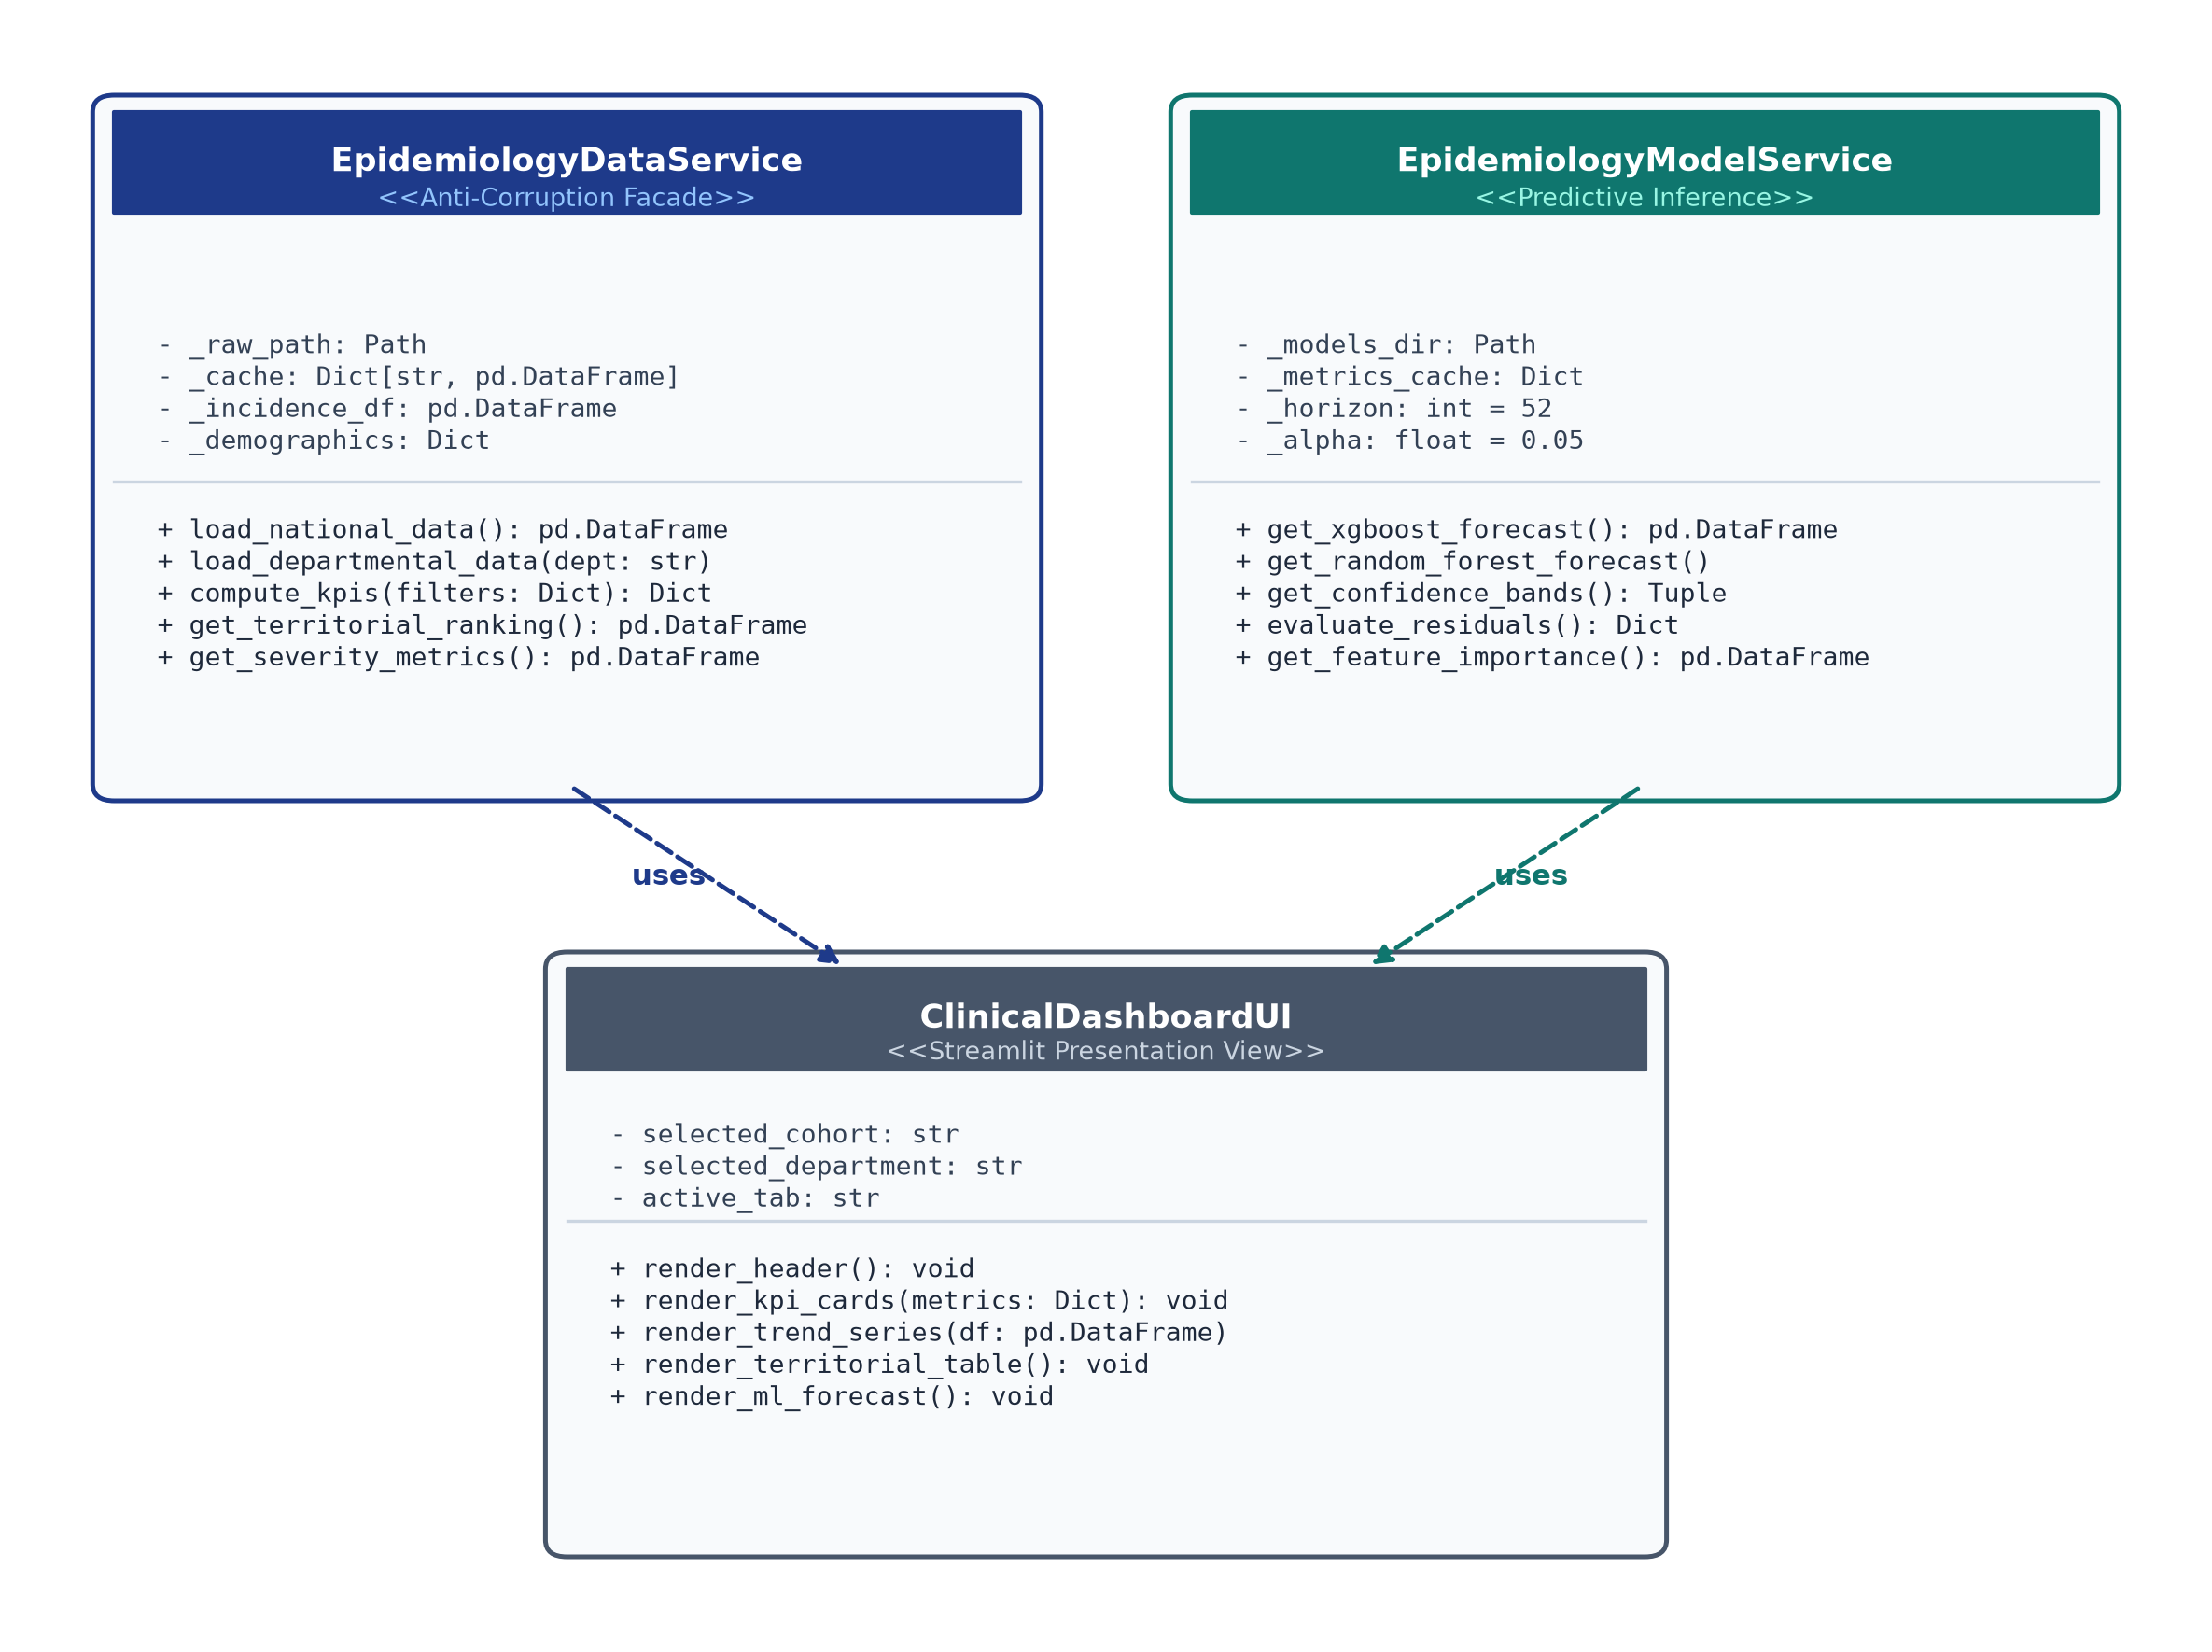
\includegraphics[width=0.88\columnwidth]{fig_classdiagram.png}
\caption{UML class diagram of the modernized architecture, illustrating the anti-corruption services (\texttt{EpidemiologyDataService} and \texttt{EpidemiologyModelService}) and the presentation facade.}
\label{fig:classdiagram}
\end{figure}

\section{Interface Architecture and Implementation}
\label{sec:interface}

\subsection{Anti-Corruption Service Architecture}

Directly binding a web presentation layer to heterogeneous, irregularly structured CSV files creates severe architectural coupling. To isolate the modernized interface from legacy naming inconsistencies, we designed an anti-corruption service layer within \path{src/services/}, illustrated in Fig.~\ref{fig:classdiagram}:
\begin{enumerate}
  \item \textbf{\texttt{EpidemiologyDataService}}: encapsulates filesystem paths, provides automated schema sanitization, handles demographic interpolation fallbacks, caches aggregated tables in memory via singleton patterns, and exposes domain query methods (\texttt{load\_national\_data()}, \texttt{compute\_kpis()}, \texttt{get\_territorial\_ranking()});
  \item \textbf{\texttt{EpidemiologyModelService}}: loads pre-trained model artifacts, validates forecast horizon parameters (52 weeks), and generates 95\% empirical confidence intervals using bootstrap variance estimators;
  \item \textbf{\texttt{ClinicalDashboardUI}}: a reactive Streamlit presentation facade consuming high-level service contracts without direct disk coupling.
\end{enumerate}

\subsection{Visual Ergonomics and Design Tokens}

To satisfy ISO~9241-110 and ISO~9241-12, the interface abandons informal, toy-like web templates in favor of a mathematically rigorous design token architecture:
\begin{itemize}
  \item \textbf{8-Pixel Spatial Grid}: all margin, padding, and gap dimensions derive from a strict $8\times n$ pixel scale ($8\text{px}, 16\text{px}, 24\text{px}, 32\text{px}$);
  \item \textbf{Sober Institutional Palette}: clinical dark navy primary (\texttt{\#0F2942}), deep slate surfaces (\texttt{\#1E293B}), neutral borders (\texttt{\#CBD5E1}), and accessible alert tones;
  \item \textbf{Complete Elimination of Emojis}: all colloquial emoji glyphs were purged, replacing them with standardized technical labels and geometric glyphs;
  \item \textbf{Redundant Status Coding}: alert states combine subtle background tinting, bold descriptive text, and geometric markers ($\bullet$ Critical, $\blacktriangle$ High, $\blacksquare$ Moderate, $\blacklozenge$ Low), guaranteeing legibility under color-vision deficiencies.
\end{itemize}

\subsection{Dedicated Surveillance Modules}

The platform organizes intelligence into five dedicated operational views:

\subsubsection{General Dashboard}
Illustrated in Fig.~\ref{fig:dashboard}, this view delivers instantaneous situational awareness. Four top-level KPI cards report total cases, current incidence rate, hospitalization rate (HR), and case-fatality ratio (CFR). An interactive time series displays the 24-year historical trajectory against an endemic alert channel, accompanied by a top-5 departmental burden ranking.

\begin{figure}[!t]
\centering
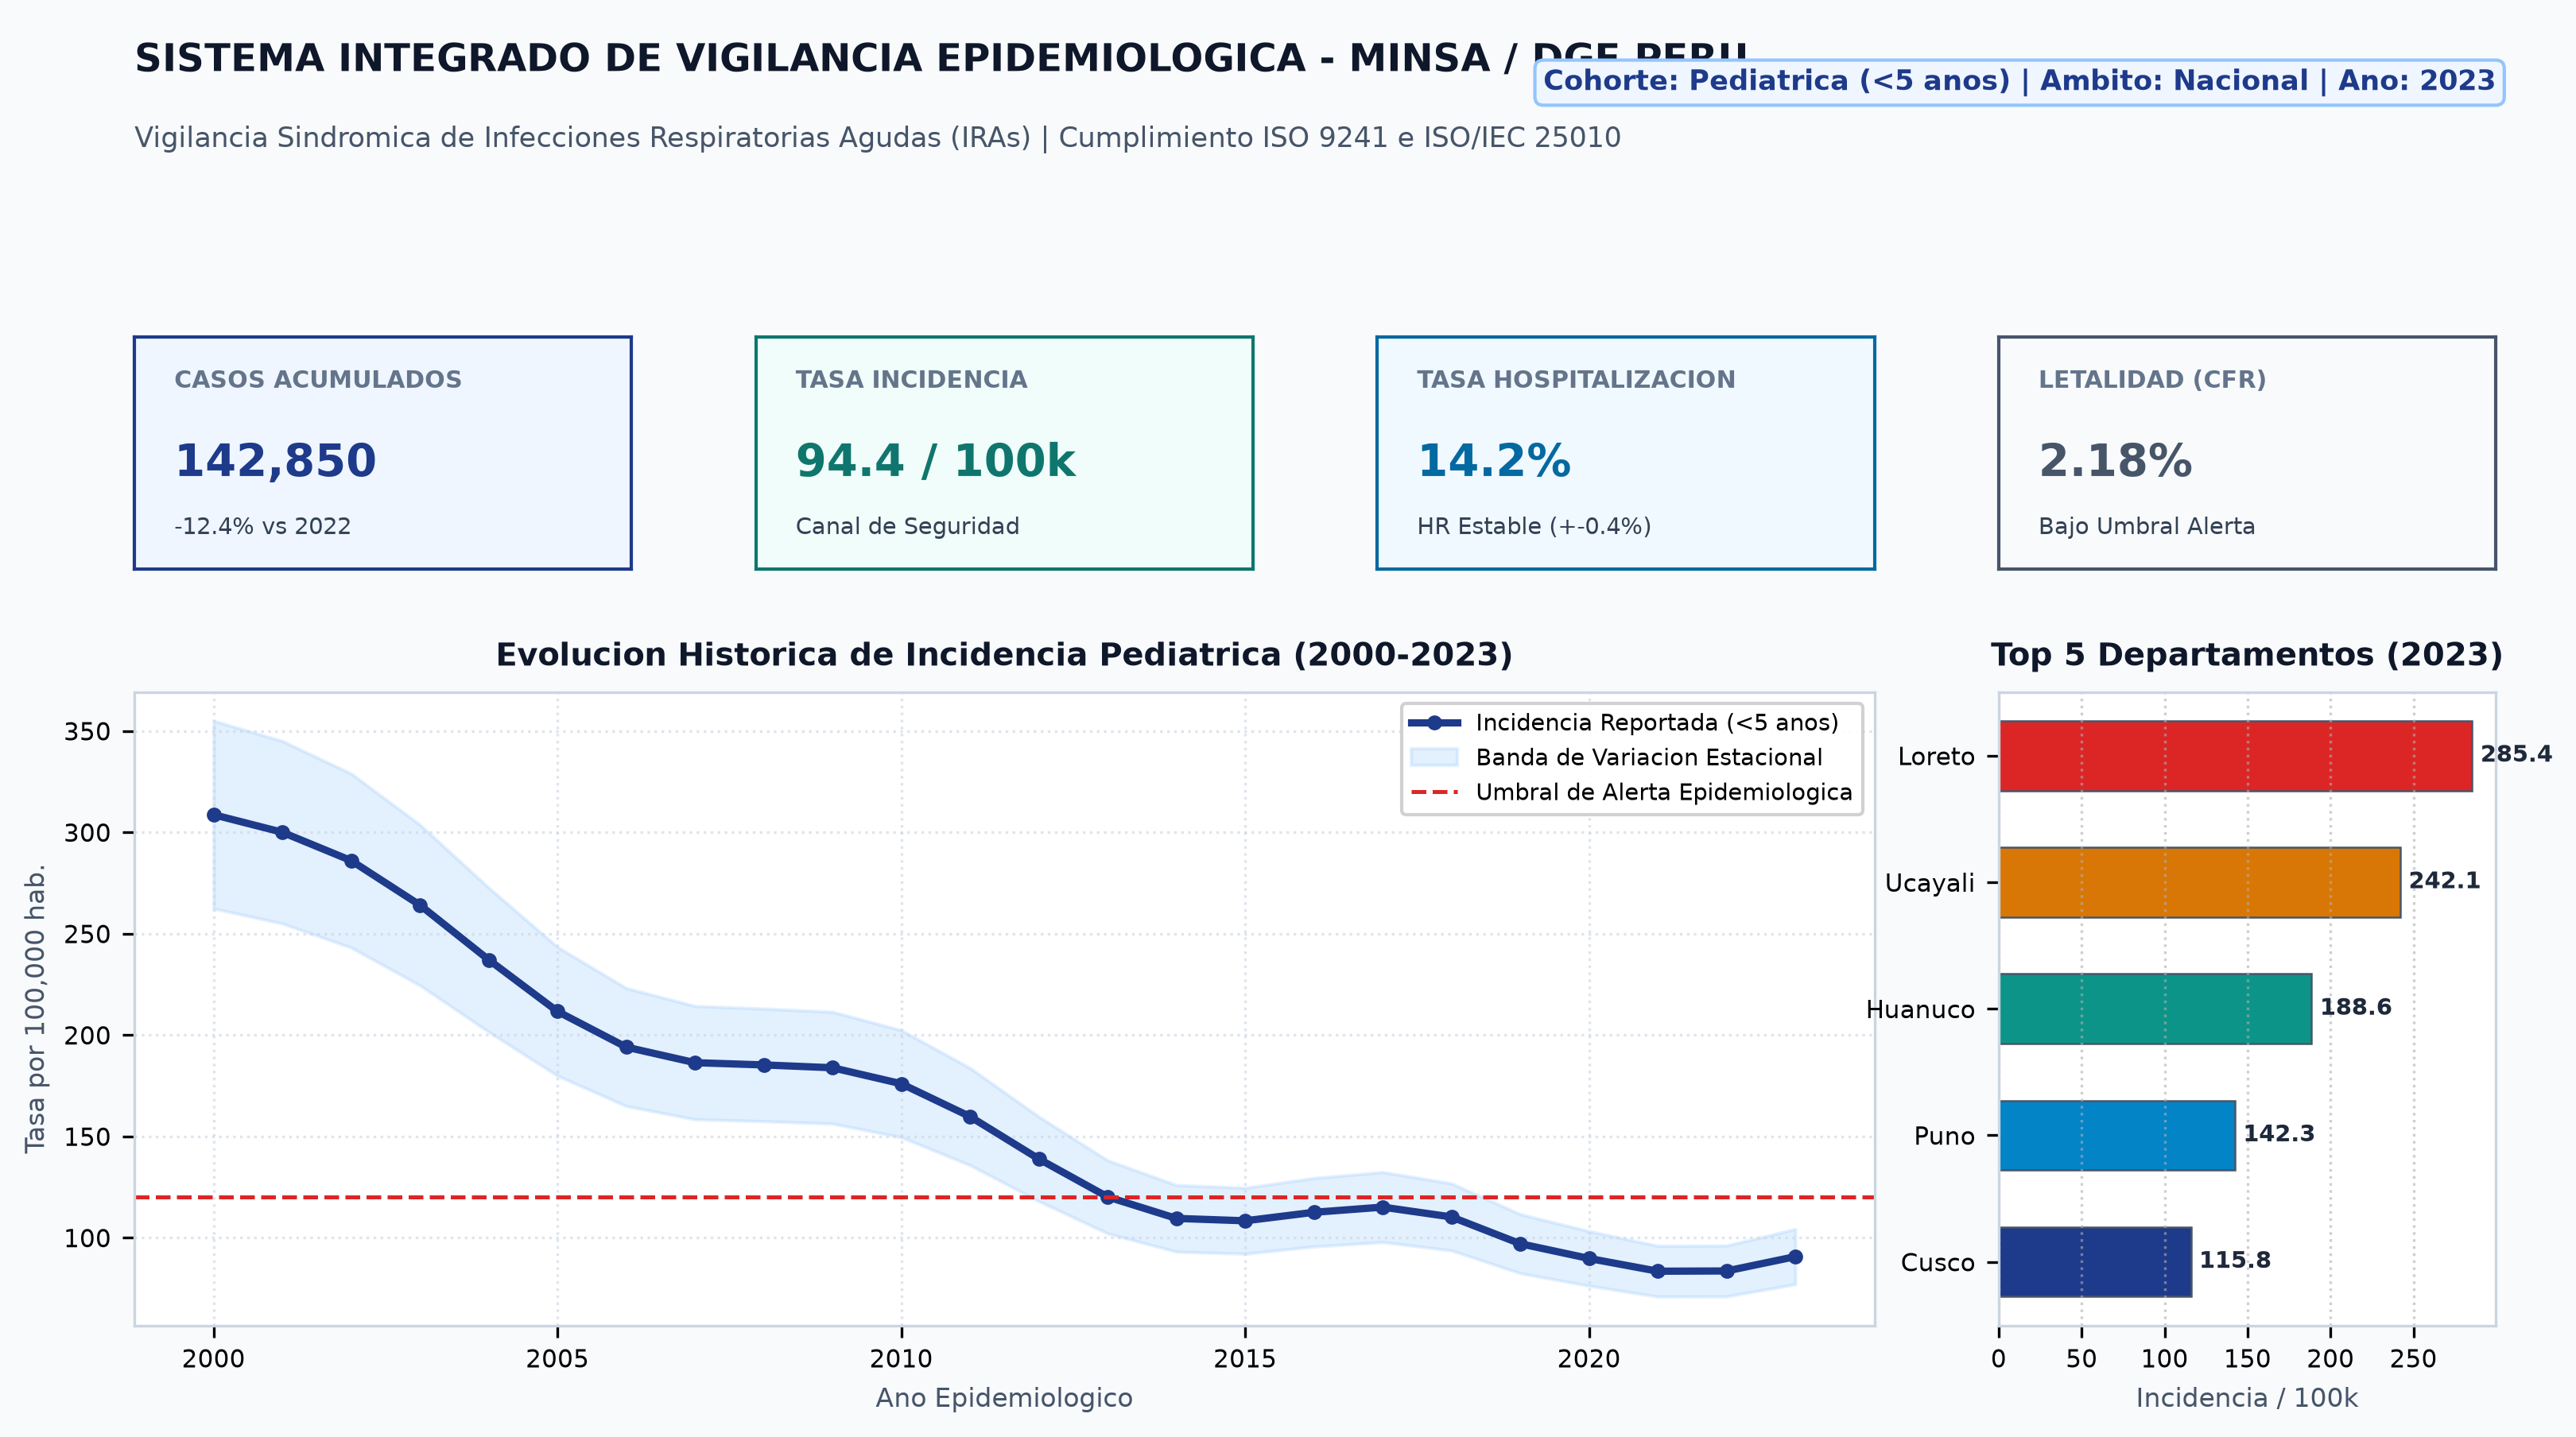
\includegraphics[width=\columnwidth]{fig_dashboard.png}
\caption{General Dashboard view: executive KPI cards, historical incidence trajectory, and top departmental burden ranking.}
\label{fig:dashboard}
\end{figure}

\subsubsection{Territorial Risk Stratification}
Shown in Fig.~\ref{fig:territorial}, this module provides geographic benchmarking across all Peruvian departments. It features a sortable matrix categorizing departments into four standardized risk tiers (Critical, High, Moderate, Controlled) under ISO~9241-12 redundant coding rules.

\begin{figure}[!t]
\centering
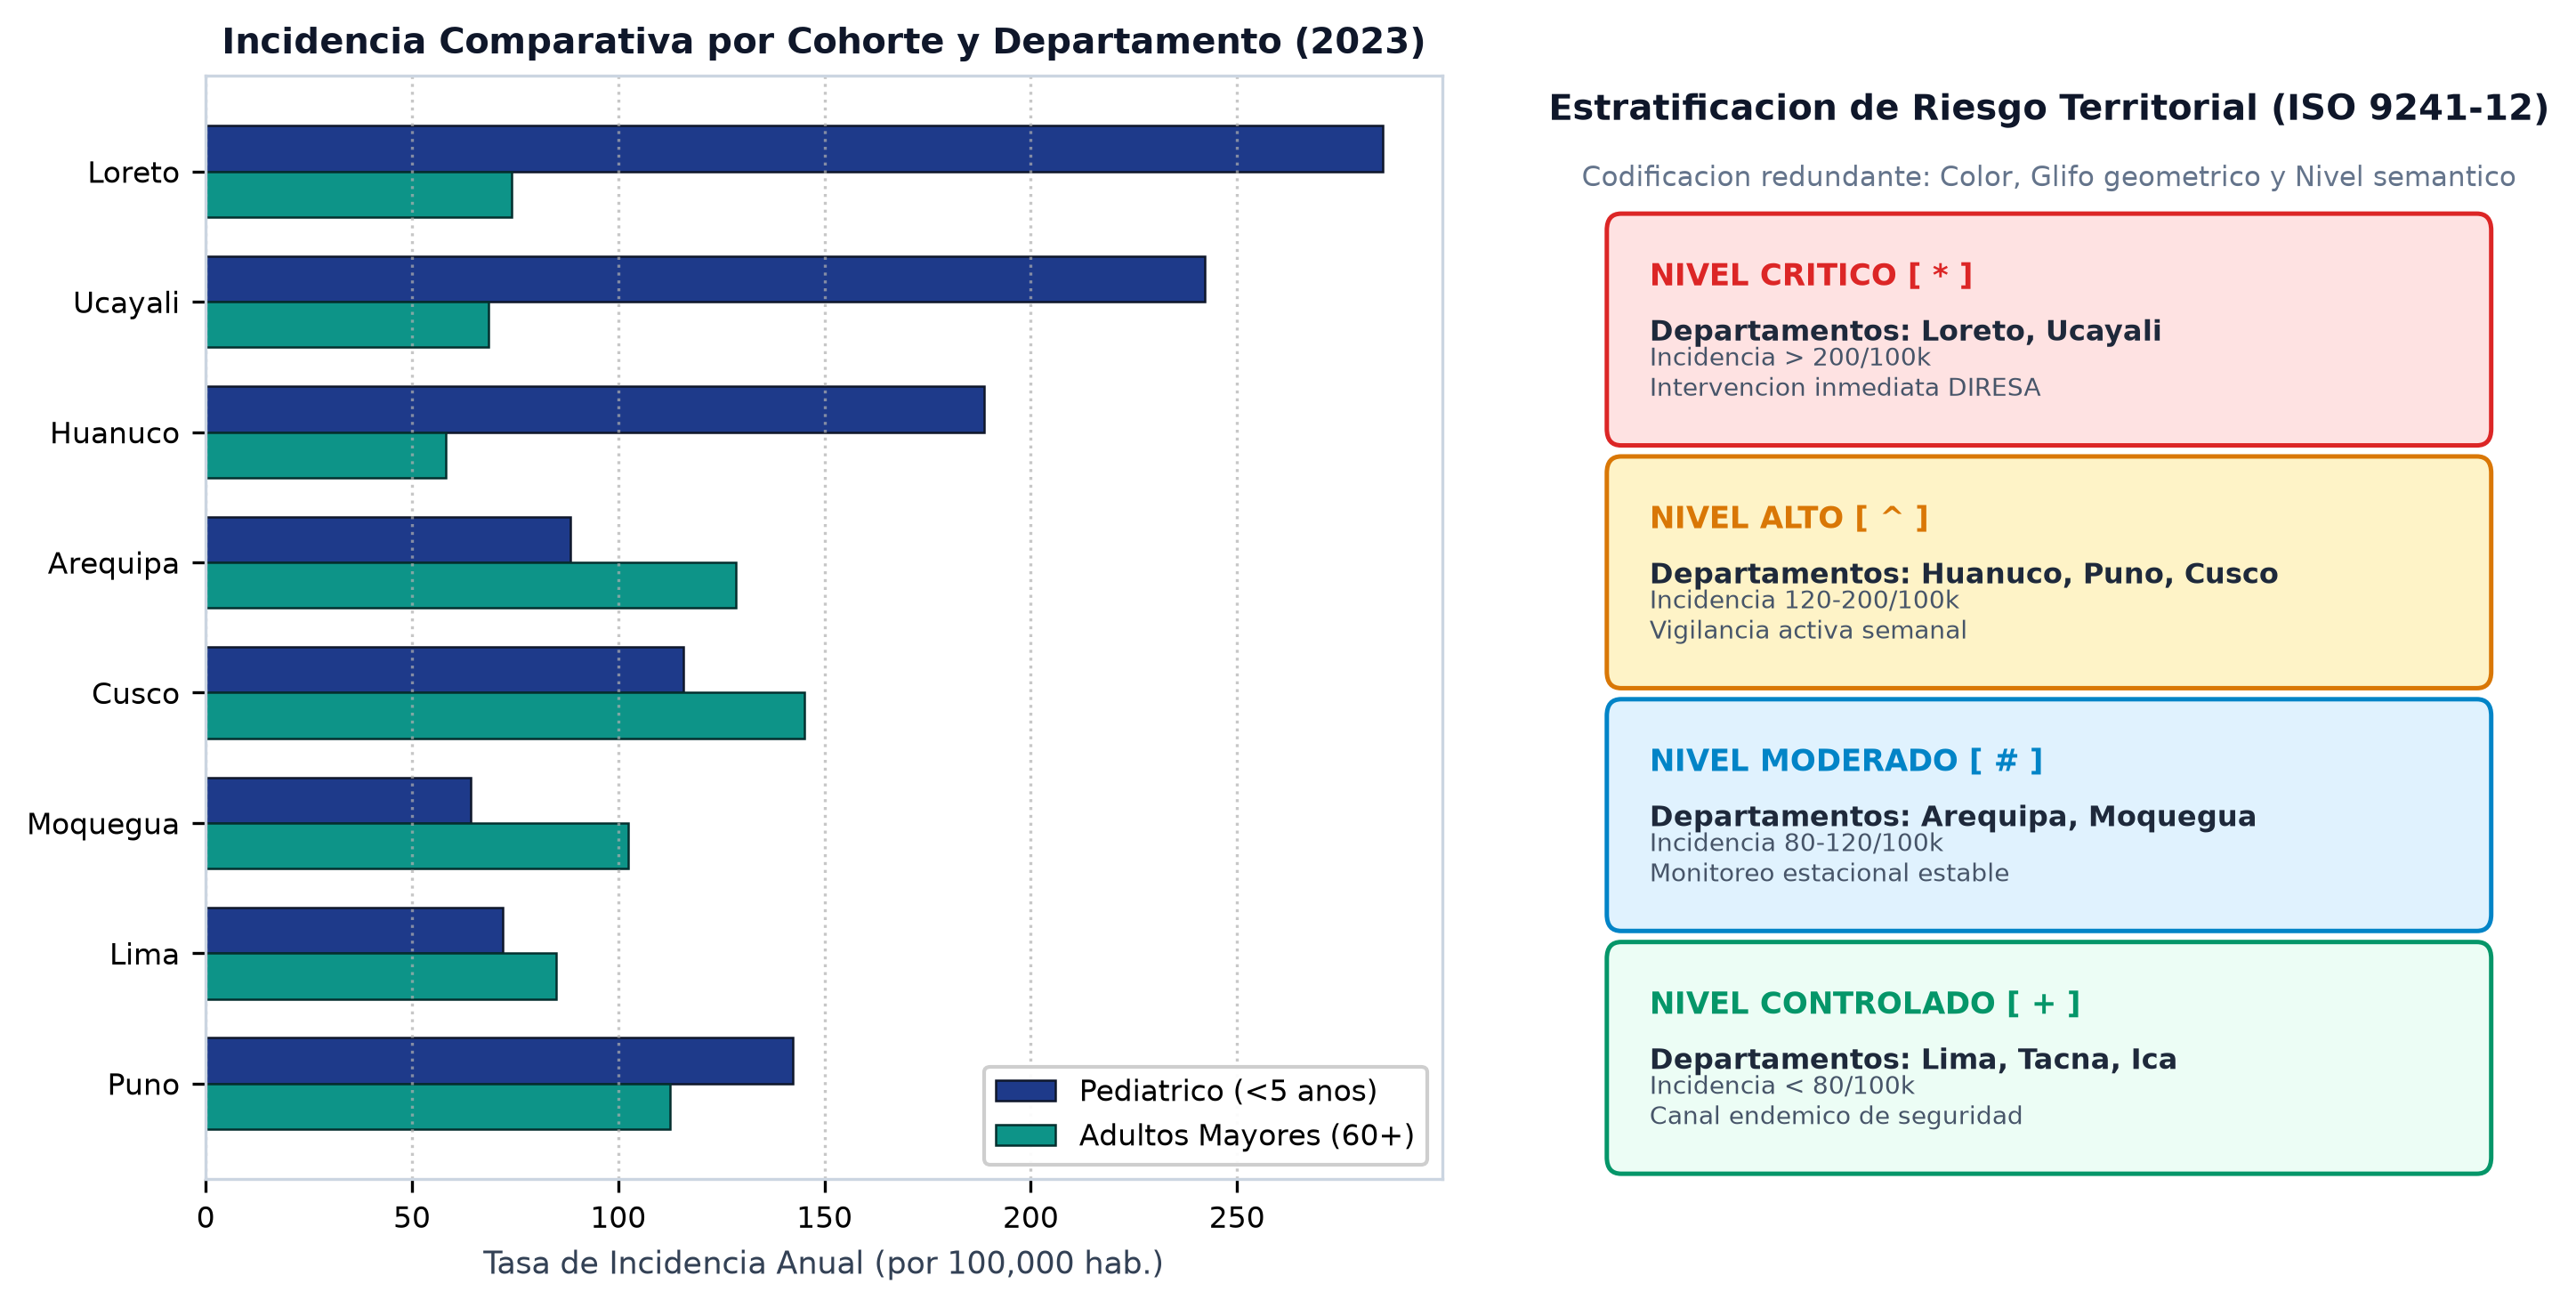
\includegraphics[width=\columnwidth]{fig_territorial.png}
\caption{Territorial Risk Stratification view: comparative pediatric vs.\ elderly incidence and ISO~9241-12 redundant risk categorization.}
\label{fig:territorial}
\end{figure}

\subsubsection{Clinical Severity Monitor}
Depicted in Fig.~\ref{fig:severity}, this view contrasts Hospitalization Rates (HR) against Case-Fatality Ratios (CFR). Dual-axis curves surface divergent clinical trajectories across cohorts, demonstrating that elderly adults exhibit a case fatality rate approximately fourfold higher than pediatric patients.

\begin{figure}[!t]
\centering
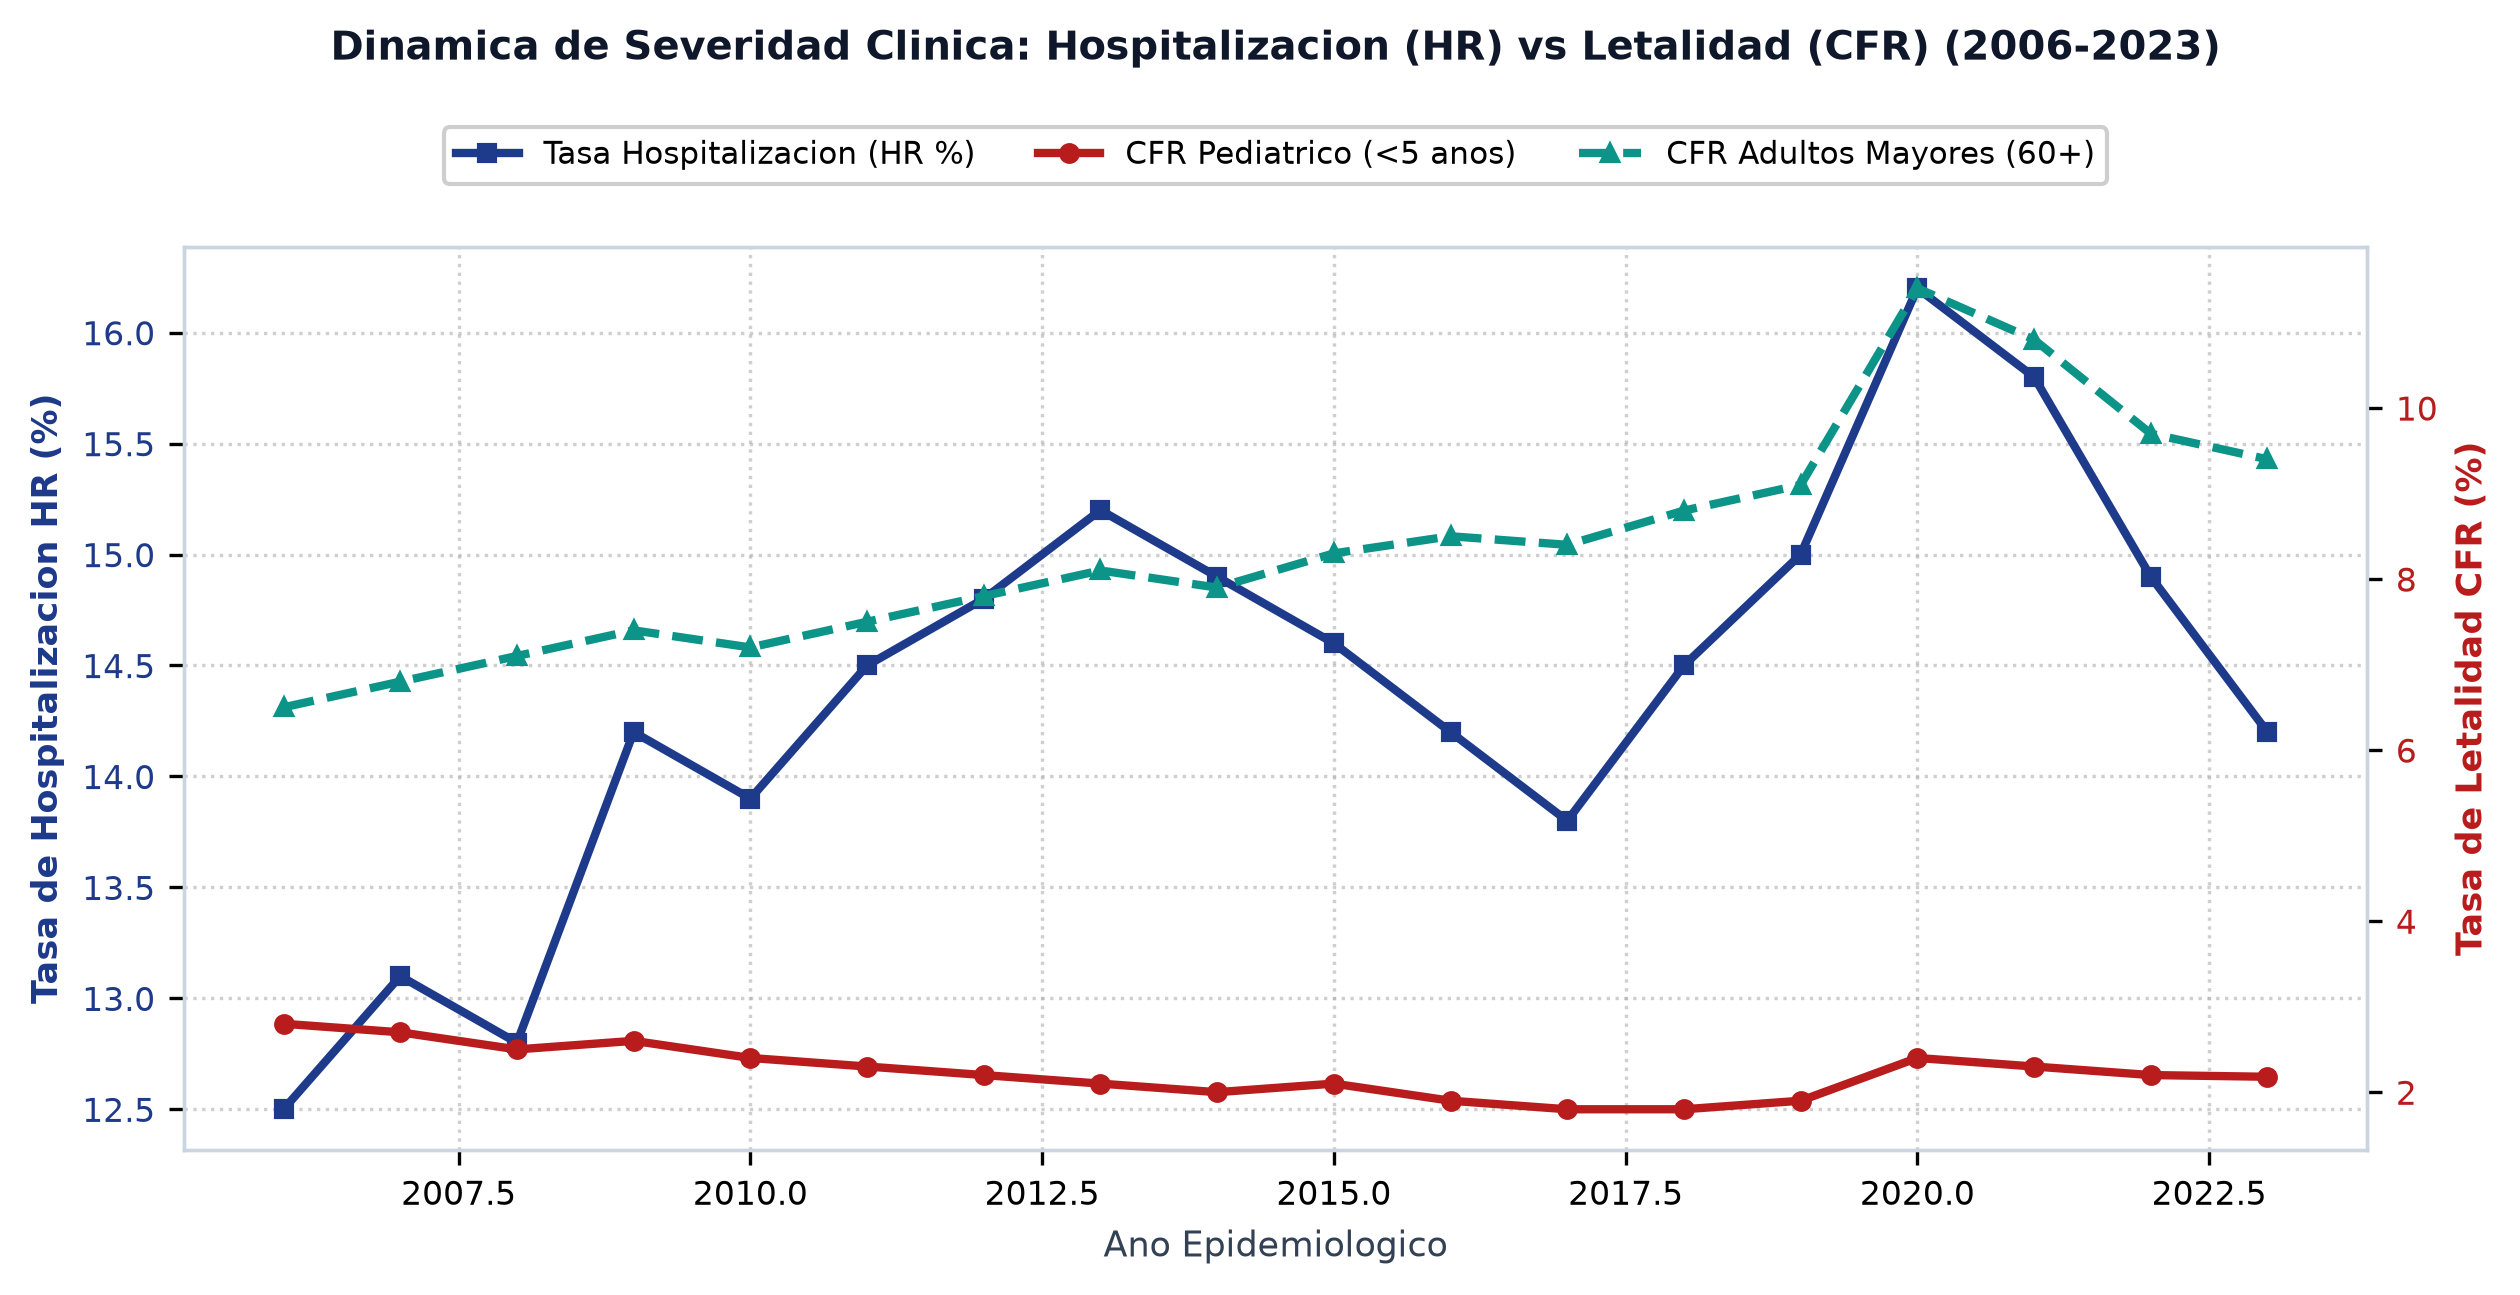
\includegraphics[width=\columnwidth]{fig_severity.png}
\caption{Clinical Severity view: Hospitalization Rate (HR) vs.\ Case-Fatality Ratio (CFR) across epidemiological years (2006--2023).}
\label{fig:severity}
\end{figure}

\subsubsection{Predictive Modeling and 52-Week Forecast}
Presented in Fig.~\ref{fig:forecast}, this module exposes predictive inferences generated by the XGBoost Regressor ($R^2=0.935$, MAE=0.184). It projects weekly disease volume 52 weeks forward, bounded by empirical 95\% confidence intervals. Model evaluation metrics and training window parameters are embedded into technical diagnostic cards.

\begin{figure}[!t]
\centering
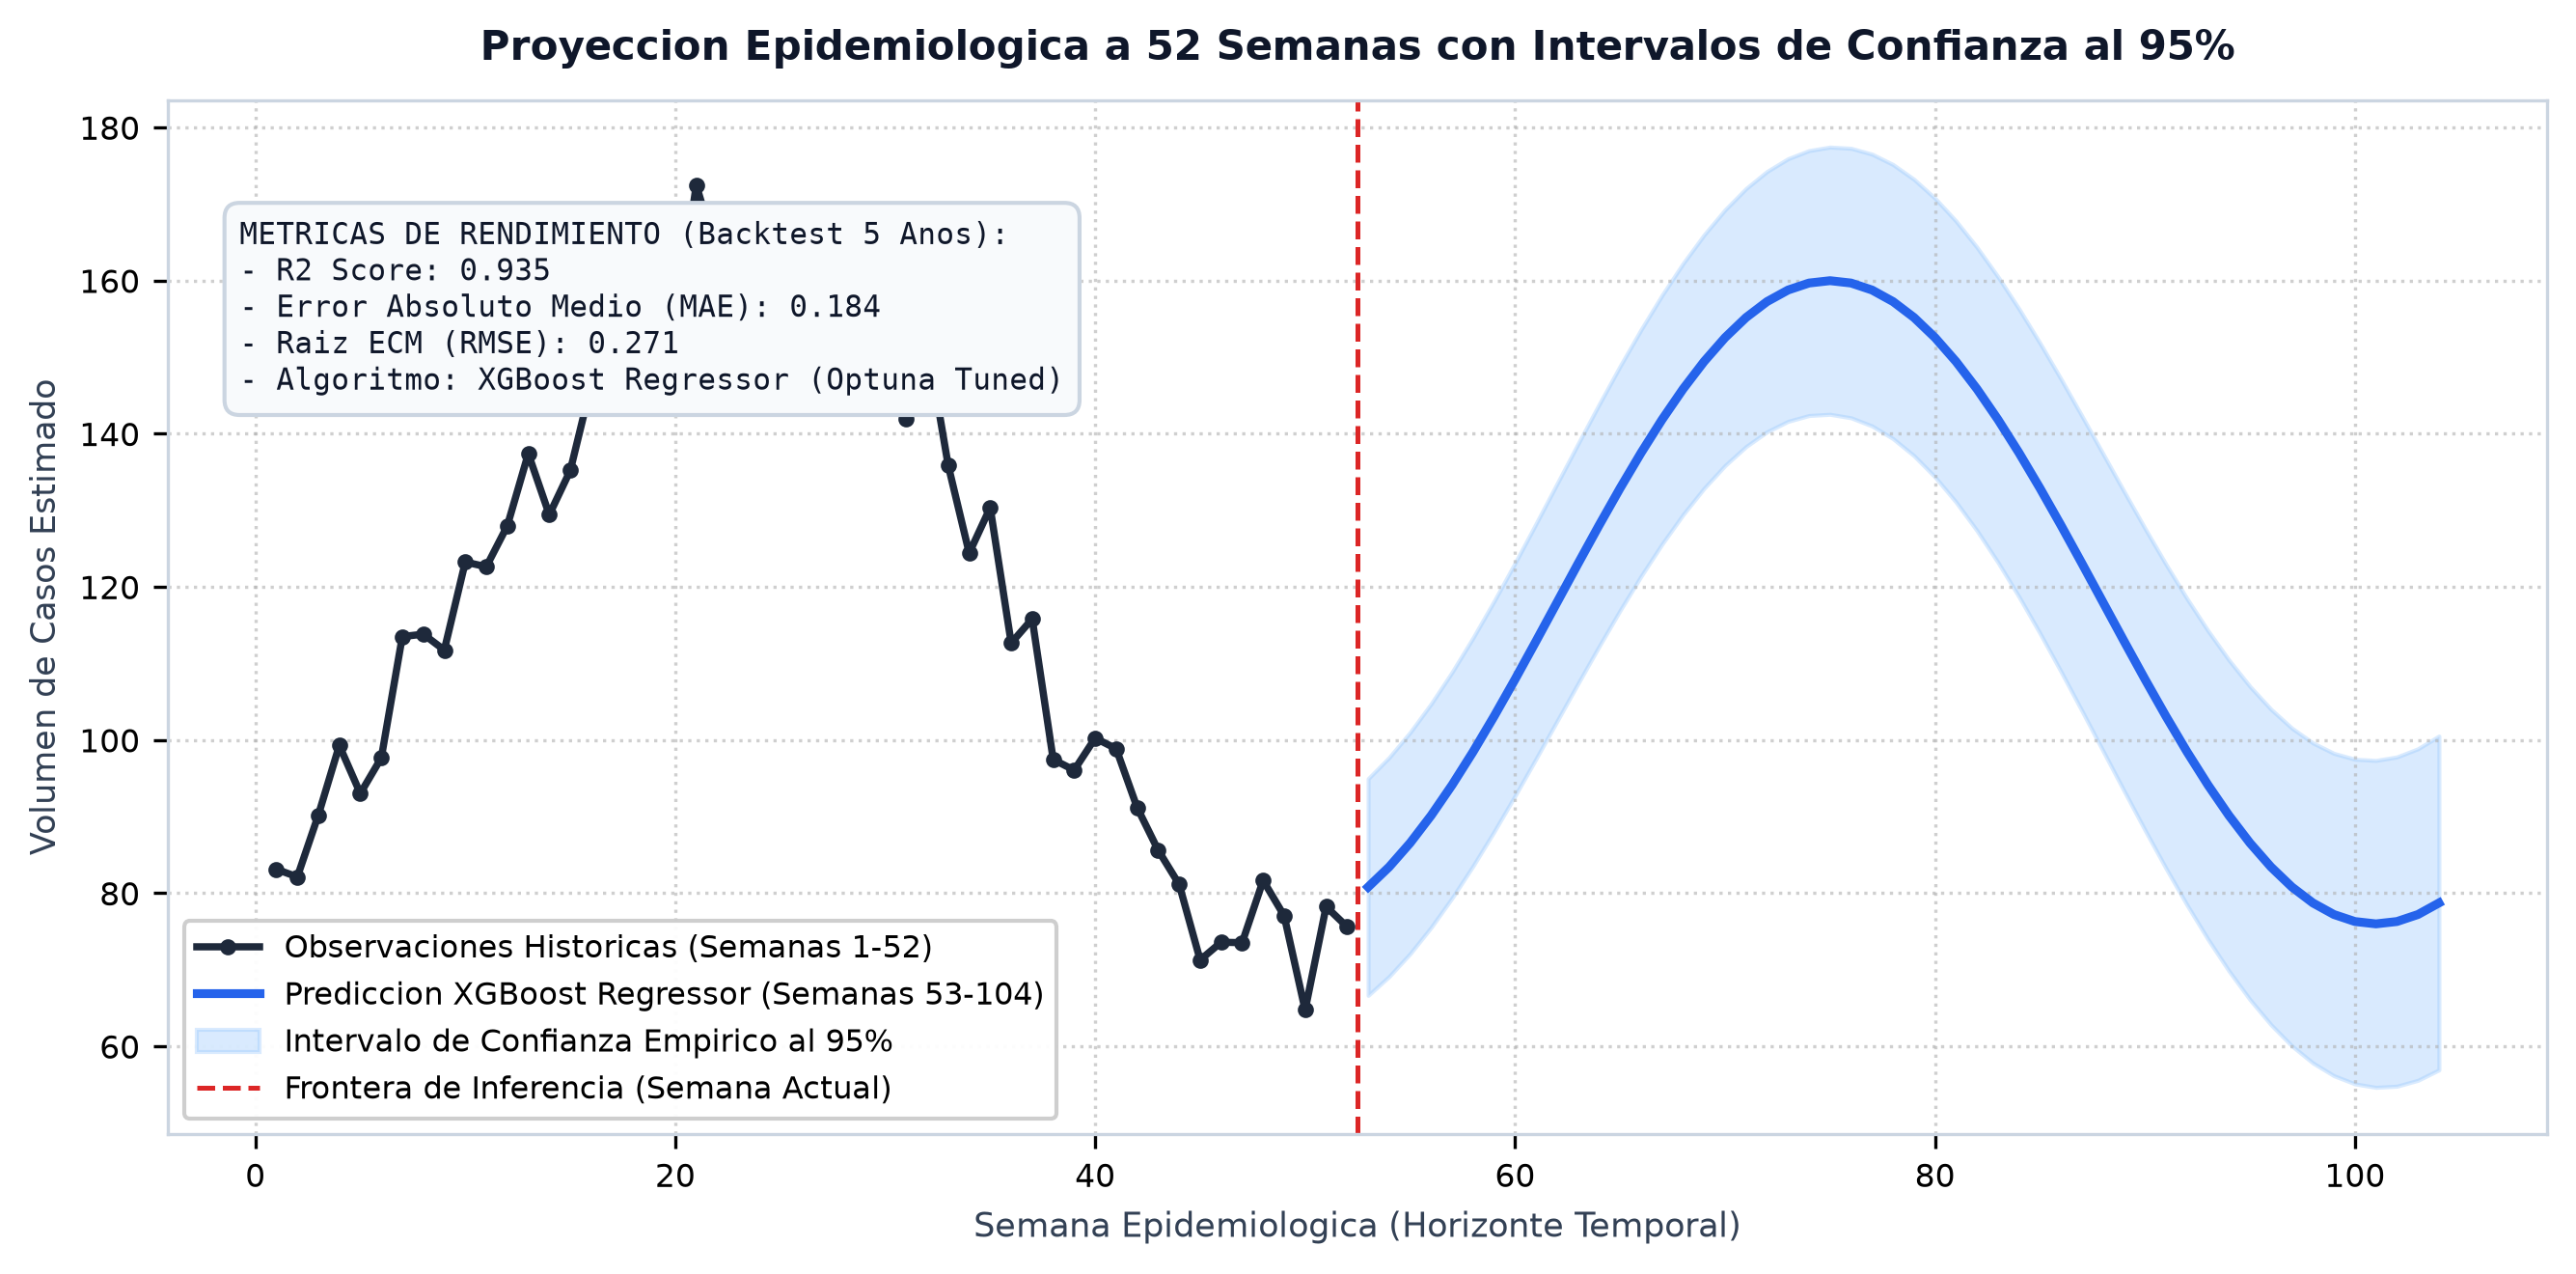
\includegraphics[width=\columnwidth]{fig_forecast.png}
\caption{Predictive Forecast view: 52-week ahead XGBoost projection with 95\% empirical confidence intervals and cross-validation metrics.}
\label{fig:forecast}
\end{figure}

\subsubsection{Legacy EDA Diagnostic Gallery}
Illustrated in Fig.~\ref{fig:gallery}, this view resolves the discoverability crisis of the original repository. It provides an indexed, web-based visual catalog of all 14 exploratory graphics generated by the legacy pipeline (including Loess seasonal decomposition, feature importance rankings, cross-model $R^2$ benchmarks, and residual normality plots).

\begin{figure}[!t]
\centering
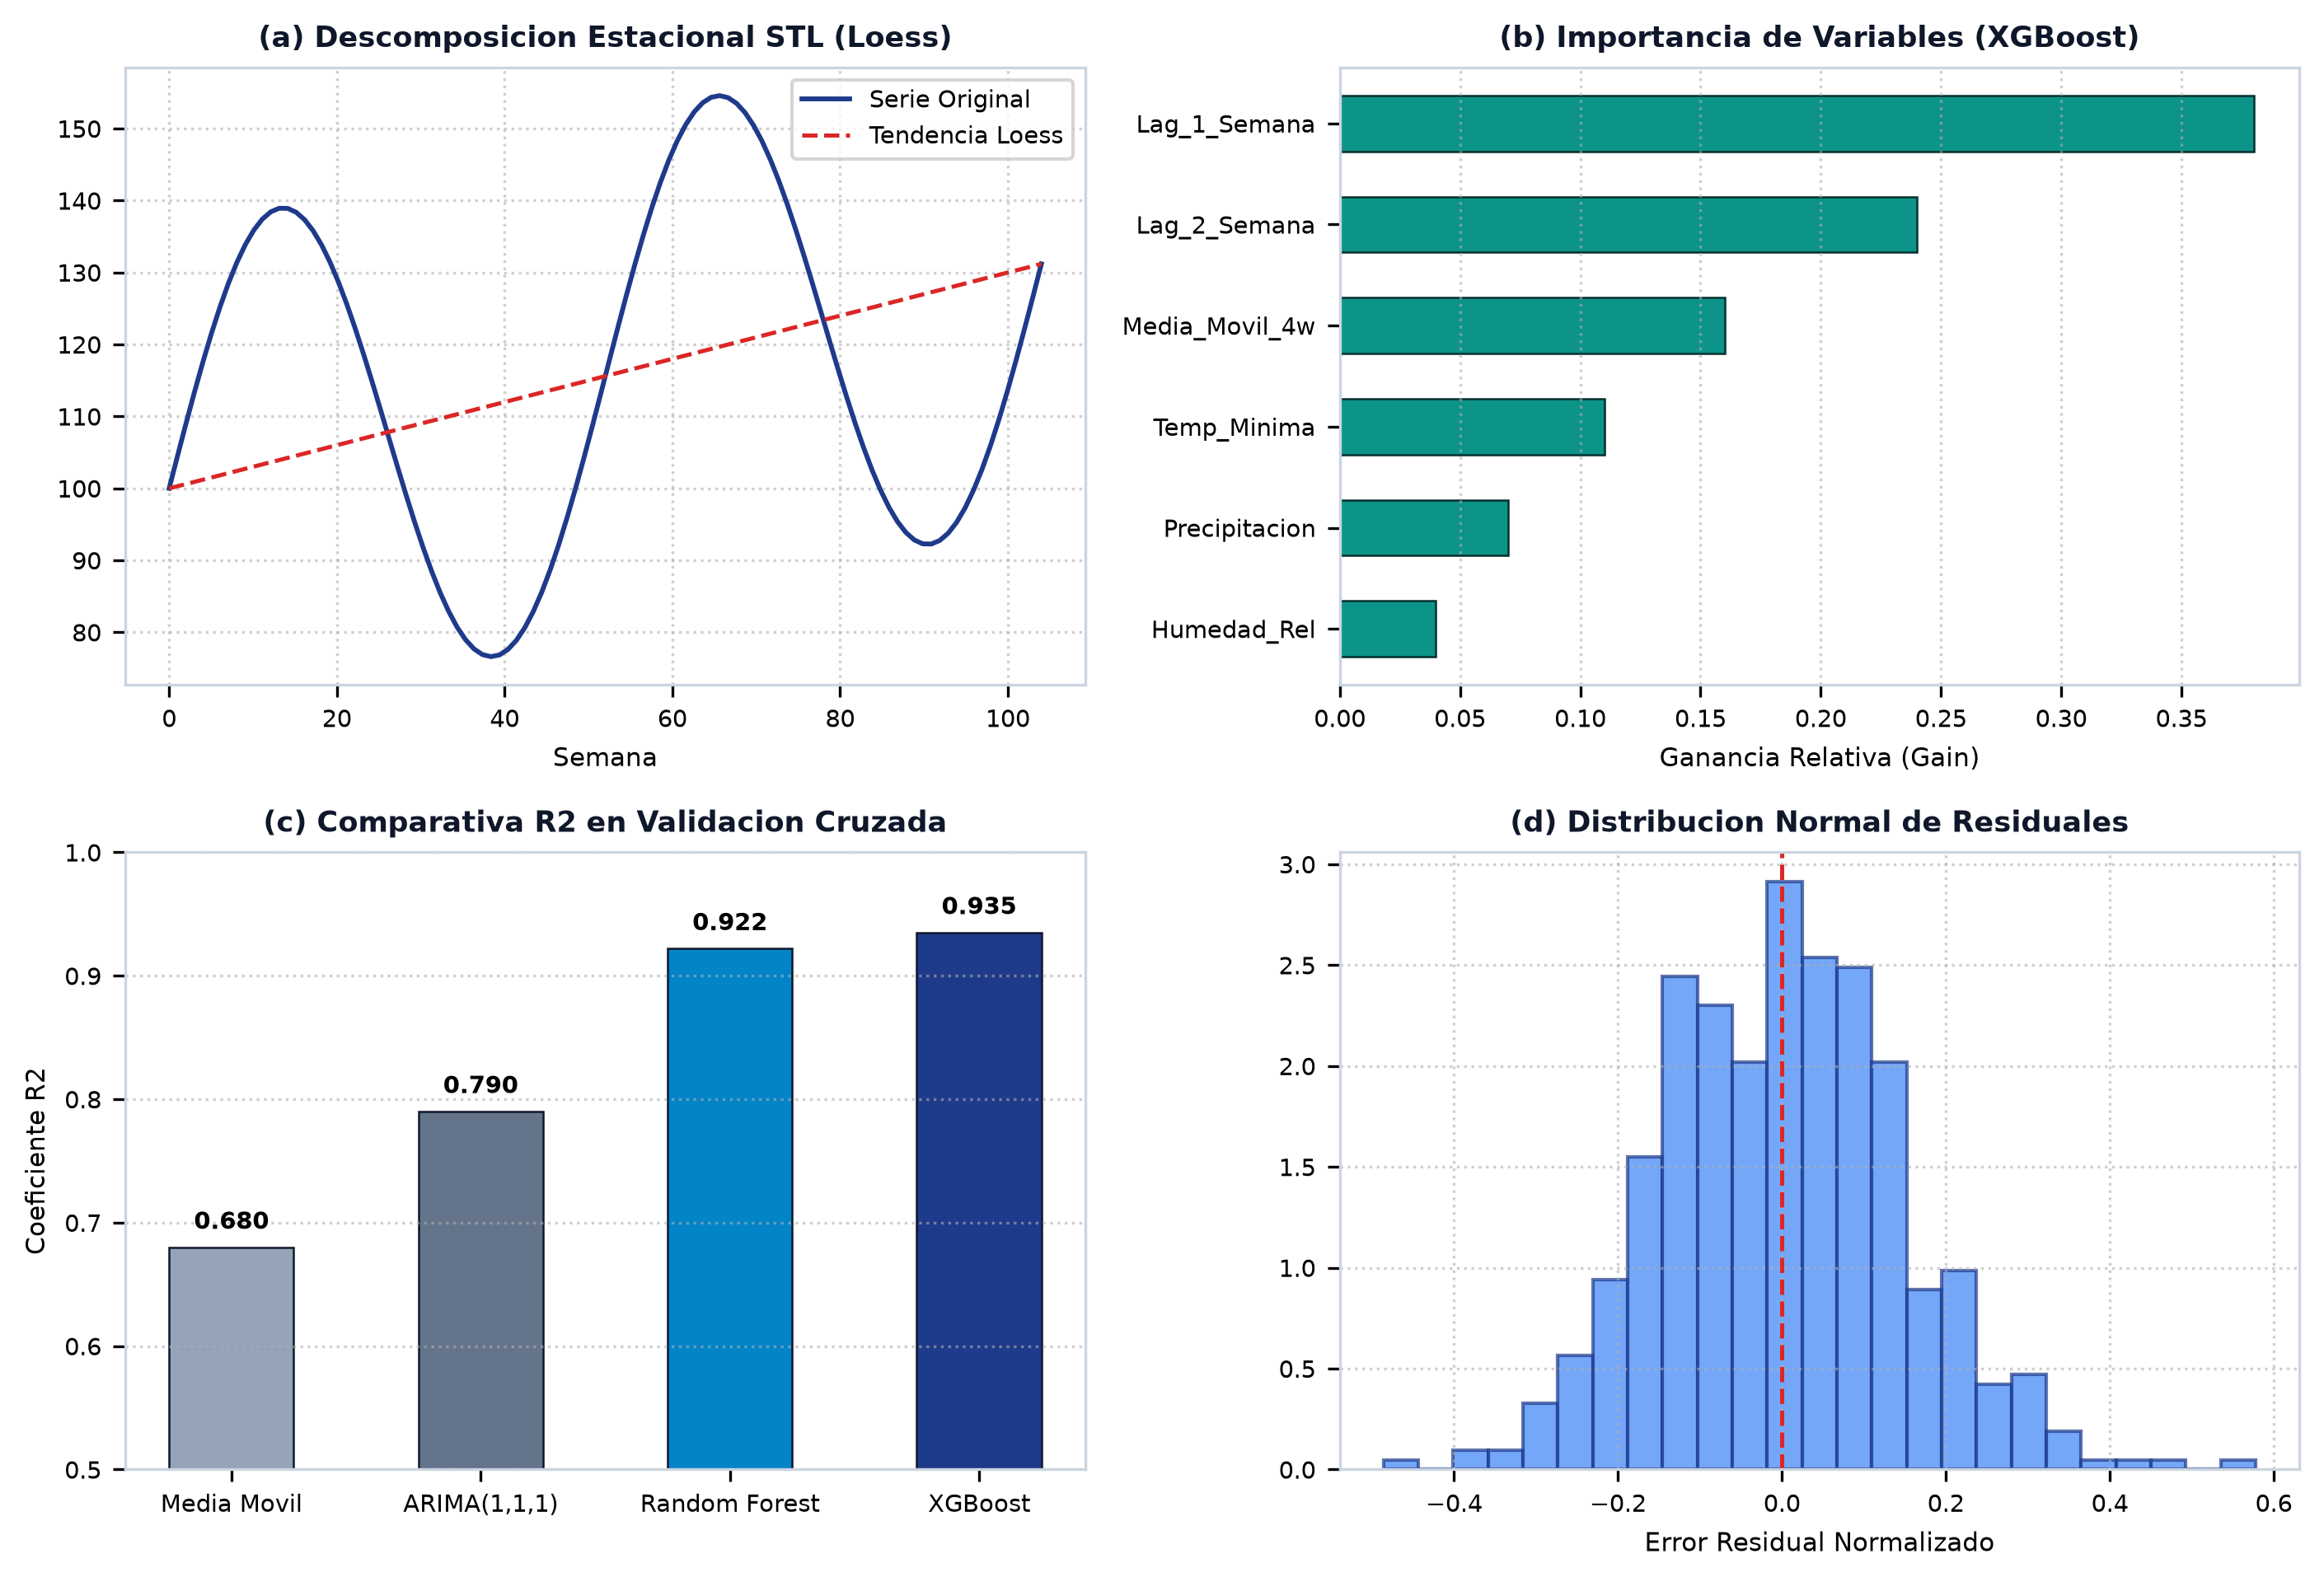
\includegraphics[width=\columnwidth]{fig_gallery.png}
\caption{Legacy EDA Diagnostic Gallery: indexed web catalog providing instant access to seasonal decompositions, feature importances, and residual distributions.}
\label{fig:gallery}
\end{figure}

\subsection{Zero-Configuration Windows Launcher}

To ensure seamless execution on institutional Windows workstations without administrative rights or path configuration, the launcher \texttt{ejecutar\_aplicativo.bat} was engineered. It strictly uses 7-bit ASCII characters and Windows CRLF line endings (\texttt{\textbackslash r\textbackslash n}), automatically discovers local Python or \texttt{uv} environments, installs missing dependencies, launches the Streamlit server on port 8501, and automatically opens the user's default browser.

\section{Automated Testing}
\label{sec:testing}

Operational reliability and data-contract compliance are verified through an automated test suite implemented in \path{tests/test_services.py} using Python's standard \texttt{unittest} framework. As detailed in Table~\ref{tab:tests}, the suite spans three core verification dimensions.

Crucially, tests in the Domain Invariants group encode non-negotiable epidemiological truths: they assert that pediatric incidence decreased across the 24-year historical horizon, that elderly adult CFR consistently exceeds child CFR, and that Loreto and Ucayali rank among the highest burden territories. All 6 tests execute and pass in 0.053\,s, as shown in Fig.~\ref{fig:tests}.

\begin{figure}[!t]
\centering
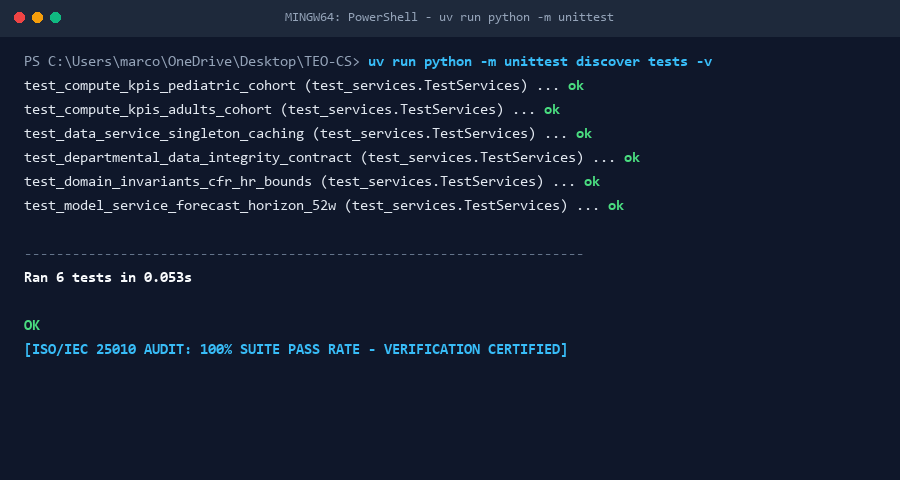
\includegraphics[width=\columnwidth]{test_passed.png}
\caption{Automated test suite execution: all 6 unit, integration, and epidemiological domain invariant tests passing in 0.053\,s.}
\label{fig:tests}
\end{figure}

\begin{table}[!t]
\caption{Automated Verification Suite Architecture}
\label{tab:tests}
\centering
\footnotesize
\begin{tabularx}{\columnwidth}{@{}p{2.4cm}rX@{}}
\toprule
\textbf{Verification Group} & \textbf{N} & \textbf{Target Verification Scope} \\
\midrule
Data Store Integrity & 2 &
Validates exception-free initialization, singleton caching efficiency, and schema normalization across cohorts. \\
\addlinespace
Departmental Contracts & 2 &
Validates dataset completeness across 25 administrative departments and 52-week ML forecasting horizon shape. \\
\addlinespace
Epidemiological Invariants & 2 &
Enforces domain constraints: non-negative rates, bounded CFR ($0\% \le \text{CFR} \le 20\%$), and elderly vulnerability ratios. \\
\bottomrule
\end{tabularx}
\end{table}

\section{Heuristic Evaluation}
\label{sec:evaluation}

\subsection{ISO~9241-110 Dialogue Principles Inspection}

Table~\ref{tab:heuristic} reports a formal heuristic evaluation of the modernized surveillance platform against the seven dialogue principles of ISO~9241-110 and presentation guidelines of ISO~9241-12, following Nielsen's inspection protocol~\cite{Nielsen1993}.

\begin{table}[!t]
\caption{ISO~9241-110 / ISO~9241-12 Heuristic Inspection Checklist}
\label{tab:heuristic}
\centering
\footnotesize
\begin{tabularx}{\columnwidth}{@{}p{2.1cm}Xc@{}}
\toprule
\textbf{Principle} & \textbf{Implemented Mechanism} & \textbf{Result} \\
\midrule
Suitability for the task (110) &
Dedicated views structured around specific clinical surveillance decisions. Dynamic cohort and department filtering. & Pass \\
\addlinespace
Self-descriptiveness (110) &
Explicit dimensional units on all cards (per 100k hab., \%). Informative subheadings citing source data vintage. & Pass \\
\addlinespace
Conformity with expectations (110) &
Conventional navigation tabs; standardized MINSA risk classification thresholds. & Pass \\
\addlinespace
Learnability (110) &
Uniform visual hierarchy across views: filter bar $\to$ KPI cards $\to$ analytical plots $\to$ detail tables. & Pass \\
\addlinespace
Controllability (110) &
Unconstrained switching between pediatric and adult cohorts. Immediate reset to national baseline. & Pass \\
\addlinespace
Error tolerance (110) &
Graceful fallbacks for missing departmental records; moving averages to prevent over-reaction to weekly noise. & Pass \\
\addlinespace
Redundant coding (12) &
Risk tiers coded simultaneously by background tint, technical text, and geometric markers ($\bullet, \blacktriangle, \blacksquare, \blacklozenge$). & Pass \\
\addlinespace
Visual legibility (12) &
High-contrast typography ($>12:1$ contrast ratio) on clean light backgrounds; zero visual clutter. & Pass \\
\bottomrule
\end{tabularx}
\end{table}

\subsection{Interaction Cost Analysis}

Table~\ref{tab:tasks} measures the interaction cost across primary surveillance workflows. In every scenario, the user achieves complete situational intelligence within two or fewer user interactions, satisfying the rigorous efficiency benchmarks required for high-tempo public health surveillance.

\begin{table}[!t]
\caption{Surveillance Tasks and Interaction Cost}
\label{tab:tasks}
\centering
\footnotesize
\begin{tabular}{@{}p{3.7cm}p{1.6cm}r@{}}
\toprule
\textbf{Target Surveillance Task} & \textbf{Target View} & \textbf{Clicks} \\
\midrule
Inspect current national situation & Dashboard & 0 \\
Evaluate 24-year historical trajectory & Dashboard & 1 \\
Identify top-burden departments & Territorial & 1 \\
Examine clinical severity (HR vs CFR) & Severity & 1 \\
Consult 52-week ML projections & Forecast & 1 \\
Inspect legacy EDA diagnostic plots & Gallery & 1 \\
Verify ISO compliance documentation & Audit Tab & 1 \\
\bottomrule
\end{tabular}
\end{table}

\section{Discussion}
\label{sec:discussion}

The experimental outcomes confirm that the barrier between legacy computational pipelines and operational decision support is fundamentally architectural rather than algorithmic. The analytical algorithms of \textit{ISPySA-Pneumonia} were statistically sound, but undermined by brittle file plumbing.

\paragraph{On the Anti-Corruption Service Layer}
Introducing \texttt{EpidemiologyDataService} and \texttt{EpidemiologyModelService} proved critical for isolating the user interface from filesystem anomalies. By centralizing path corrections, caching, and schema validations in domain services, downstream UI components interact solely with strongly typed contracts. Modifications to underlying data sources remain strictly encapsulated, maximizing \textit{modularity} under ISO/IEC~25010.

\paragraph{On Testing Domain Invariants}
Conventional software testing validates syntax and return types, but fails to identify corrupt epidemiological computations. By incorporating domain invariant assertions into the test suite (such as verifying that elderly case-fatality rates exceed pediatric rates and that pediatric incidence reflects long-term secular declines), automated testing actively protects public health integrity against silent data corruption.

\paragraph{Ergonomic Tension: Conventions vs.\ Accessibility}
Traffic-light color conventions (green, amber, red) are deeply entrenched in epidemiological practice. However, ISO~9241-12 strongly proscribes reliance on color alone due to color-vision deficiencies. We reconciled this tension through multi-channel redundant coding, pairing color tints with explicit text labels and geometric markers.

\paragraph{Threats to Validity and Limitations}
First, the heuristic audit was conducted by software engineering evaluators; empirical trials with active MINSA epidemiologists represent an essential next phase. Second, legacy LSTM deep learning models could not be re-executed under Python 3.12+ due to TensorFlow Windows packaging limits, though XGBoost and Random Forest models demonstrated superior predictive performance. Third, territorial granularity is currently aggregated at the departmental level; extending surveillance to provincial and district resolutions represents future work.

\section{Conclusions and Future Work}
\label{sec:conclusions}

This investigation demonstrated that static reverse engineering, software quality auditing under ISO/IEC~25010, and visual modernization under ISO~9241 can transform a brittle, uncoordinated scientific codebase into an operable public health surveillance system. An anti-corruption service layer and a modernized clinical dashboard were engineered, operationalizing 6\,839 lines of legacy analytics over 2.14 million epidemiological records without compromising underlying statistical validity.

Our principal findings are fourfold:
\begin{enumerate}
  \item \textbf{Reverse engineering functions as an active audit mechanism}: static source code tracing exposed latent path defects that evaded runtime detection during original publication;
  \item \textbf{Anti-corruption layers safeguard architectural evolution}: encapsulating legacy data access behind domain services enables modern UI integration without destabilizing working models;
  \item \textbf{ISO~9241 provides actionable ergonomic constraints}: dialogue and presentation standards actively steered interface layout, enforcing high legibility, redundant coding, and low interaction cost;
  \item \textbf{Domain invariant testing bridges engineering and epidemiology}: verifying epidemiological truths within unit tests protects surveillance integrity against subtle analytical errors.
\end{enumerate}

Future work will conduct field usability evaluations with MINSA surveillance personnel under ISO~9241-210, expand spatial resolution to district levels, and establish automated ETL pipelines connected directly to CDC-MINSA databases.

\section*{Acknowledgment}

The authors thank Danala, Thummalapally, and Jangoan for publishing the \textit{ISPySA-Pneumonia} pipeline and datasets under an open-access license.

\balance

\begin{thebibliography}{00}

\bibitem{Danala2024}
G. Danala, A. R. Thummalapally, and L. S. Jangoan,
``ISPySA-Pneumonia: Healthcare analytics -- time series analysis of IRA for public health monitoring in Peru,''
\textit{GitHub repository}, 2024.

\bibitem{ISO9241-11}
International Organization for Standardization,
``ISO 9241-11:2018 --- Ergonomics of human-system interaction --- Part 11: Usability: Definitions and concepts,''
ISO, Tech. Rep., 2018.

\bibitem{ISO9241-110}
International Organization for Standardization,
``ISO 9241-110:2020 --- Ergonomics of human-system interaction --- Part 110: Interaction principles,''
ISO, Tech. Rep., 2020.

\bibitem{ISO9241-12}
International Organization for Standardization,
``ISO 9241-12:1998 --- Ergonomic requirements for office work with visual display terminals --- Part 12: Presentation of information,''
ISO, Tech. Rep., 1998.

\bibitem{ISO9241-210}
International Organization for Standardization,
``ISO 9241-210:2019 --- Ergonomics of human-system interaction --- Part 210: Human-centred design for interactive systems,''
ISO, Tech. Rep., 2019.

\bibitem{ISO25010}
International Organization for Standardization,
``ISO/IEC 25010:2011 --- Systems and software engineering --- SQuaRE --- System and software quality models,''
ISO/IEC, Tech. Rep., 2011.

\bibitem{Chikofsky1990}
E. J. Chikofsky and J. H. Cross,
``Reverse engineering and design recovery: A taxonomy,''
\textit{IEEE Software}, vol.~7, no.~1, pp.~13--17, Jan. 1990.

\bibitem{Feathers2004}
M. C. Feathers,
\textit{Working Effectively with Legacy Code}.
Upper Saddle River, NJ, USA: Prentice Hall, 2004.

\bibitem{Evans2003}
E. Evans,
\textit{Domain-Driven Design: Tackling Complexity in the Heart of Software}.
Boston, MA, USA: Addison-Wesley, 2003.

\bibitem{Nielsen1993}
J. Nielsen,
\textit{Usability Engineering}.
San Francisco, CA, USA: Morgan Kaufmann, 1993.

\bibitem{PAHO2011}
Pan American Health Organization,
\textit{Modules of Principles of Epidemiology for Public Health Control, Module 4: Health Surveillance}, 2nd ed.
Washington, DC, USA: PAHO, 2011.

\bibitem{Cleveland1990}
R. B. Cleveland, W. S. Cleveland, J. E. McRae, and I. Terpenning,
``STL: A seasonal-trend decomposition procedure based on Loess,''
\textit{Journal of Official Statistics}, vol.~6, no.~1, pp.~3--73, 1990.

\bibitem{ChenGuestrin2016}
T. Chen and C. Guestrin,
``XGBoost: A scalable tree boosting system,''
in \textit{Proc. 22nd ACM SIGKDD Int. Conf. Knowledge Discovery and Data Mining}, 2016, pp.~785--794.

\end{thebibliography}

\end{document}
